\documentclass[1p]{elsarticle_modified}
%\bibliographystyle{elsarticle-num}

%\usepackage[colorlinks]{hyperref}
%\usepackage{abbrmath_seonhwa} %\Abb, \Ascr, \Acal ,\Abf, \Afrak
\usepackage{amsfonts}
\usepackage{amssymb}
\usepackage{amsmath}
\usepackage{amsthm}
\usepackage{scalefnt}
\usepackage{amsbsy}
\usepackage{kotex}
\usepackage{caption}
\usepackage{subfig}
\usepackage{color}
\usepackage{graphicx}
\usepackage{xcolor} %% white, black, red, green, blue, cyan, magenta, yellow
\usepackage{float}
\usepackage{setspace}
\usepackage{hyperref}

\usepackage{tikz}
\usetikzlibrary{arrows}

\usepackage{multirow}
\usepackage{array} % fixed length table
\usepackage{hhline}

%%%%%%%%%%%%%%%%%%%%%
\makeatletter
\renewcommand*\env@matrix[1][\arraystretch]{%
	\edef\arraystretch{#1}%
	\hskip -\arraycolsep
	\let\@ifnextchar\new@ifnextchar
	\array{*\c@MaxMatrixCols c}}
\makeatother %https://tex.stackexchange.com/questions/14071/how-can-i-increase-the-line-spacing-in-a-matrix
%%%%%%%%%%%%%%%

\usepackage[normalem]{ulem}

\newcommand{\msout}[1]{\ifmmode\text{\sout{\ensuremath{#1}}}\else\sout{#1}\fi}
%SOURCE: \msout is \stkout macro in https://tex.stackexchange.com/questions/20609/strikeout-in-math-mode

\newcommand{\cancel}[1]{
	\ifmmode
	{\color{red}\msout{#1}}
	\else
	{\color{red}\sout{#1}}
	\fi
}

\newcommand{\add}[1]{
	{\color{blue}\uwave{#1}}
}

\newcommand{\replace}[2]{
	\ifmmode
	{\color{red}\msout{#1}}{\color{blue}\uwave{#2}}
	\else
	{\color{red}\sout{#1}}{\color{blue}\uwave{#2}}
	\fi
}

\newcommand{\Sol}{\mathcal{S}} %segment
\newcommand{\D}{D} %diagram
\newcommand{\A}{\mathcal{A}} %arc


%%%%%%%%%%%%%%%%%%%%%%%%%%%%%5 test

\def\sl{\operatorname{\textup{SL}}(2,\Cbb)}
\def\psl{\operatorname{\textup{PSL}}(2,\Cbb)}
\def\quan{\mkern 1mu \triangleright \mkern 1mu}

\theoremstyle{definition}
\newtheorem{thm}{Theorem}[section]
\newtheorem{prop}[thm]{Proposition}
\newtheorem{lem}[thm]{Lemma}
\newtheorem{ques}[thm]{Question}
\newtheorem{cor}[thm]{Corollary}
\newtheorem{defn}[thm]{Definition}
\newtheorem{exam}[thm]{Example}
\newtheorem{rmk}[thm]{Remark}
\newtheorem{alg}[thm]{Algorithm}

\newcommand{\I}{\sqrt{-1}}
\begin{document}

%\begin{frontmatter}
%
%\title{Boundary parabolic representations of knots up to 8 crossings}
%
%%% Group authors per affiliation:
%\author{Yunhi Cho} 
%\address{Department of Mathematics, University of Seoul, Seoul, Korea}
%\ead{yhcho@uos.ac.kr}
%
%
%\author{Seonhwa Kim} %\fnref{s_kim}}
%\address{Center for Geometry and Physics, Institute for Basic Science, Pohang, 37673, Korea}
%\ead{ryeona17@ibs.re.kr}
%
%\author{Hyuk Kim}
%\address{Department of Mathematical Sciences, Seoul National University, Seoul 08826, Korea}
%\ead{hyukkim@snu.ac.kr}
%
%\author{Seokbeom Yoon}
%\address{Department of Mathematical Sciences, Seoul National University, Seoul, 08826,  Korea}
%\ead{sbyoon15@snu.ac.kr}
%
%\begin{abstract}
%We find all boundary parabolic representation of knots up to 8 crossings.
%
%\end{abstract}
%\begin{keyword}
%    \MSC[2010] 57M25 
%\end{keyword}
%
%\end{frontmatter}

%\linenumbers
%\tableofcontents
%
\newcommand\colored[1]{\textcolor{white}{\rule[-0.35ex]{0.8em}{1.4ex}}\kern-0.8em\color{red} #1}%
%\newcommand\colored[1]{\textcolor{white}{ #1}\kern-2.17ex	\textcolor{white}{ #1}\kern-1.81ex	\textcolor{white}{ #1}\kern-2.15ex\color{red}#1	}

{\Large $\underline{12a_{0571}~(K12a_{0571})}$}

\setlength{\tabcolsep}{10pt}
\renewcommand{\arraystretch}{1.6}
\vspace{1cm}\begin{tabular}{m{100pt}>{\centering\arraybackslash}m{274pt}}
\multirow{5}{120pt}{
	\centering
	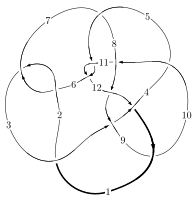
\includegraphics[width=112pt]{../../../GIT/diagram.site/Diagrams/png/1372_12a_0571.png}\\
\ \ \ A knot diagram\footnotemark}&
\allowdisplaybreaks
\textbf{Linearized knot diagam} \\
\cline{2-2}
 &
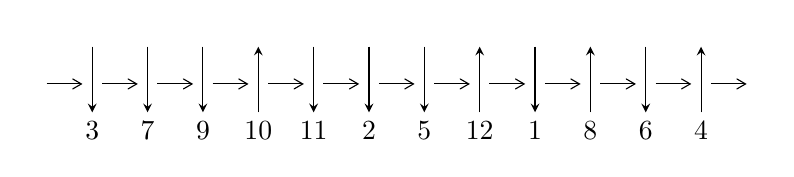
\begin{tikzpicture}[x=20pt, y=17pt]
	% nodes
	\node (C0) at (0, 0) {};
	\node (C1) at (1, 0) {};
	\node (C1U) at (1, +1) {};
	\node (C1D) at (1, -1) {3};

	\node (C2) at (2, 0) {};
	\node (C2U) at (2, +1) {};
	\node (C2D) at (2, -1) {7};

	\node (C3) at (3, 0) {};
	\node (C3U) at (3, +1) {};
	\node (C3D) at (3, -1) {9};

	\node (C4) at (4, 0) {};
	\node (C4U) at (4, +1) {};
	\node (C4D) at (4, -1) {10};

	\node (C5) at (5, 0) {};
	\node (C5U) at (5, +1) {};
	\node (C5D) at (5, -1) {11};

	\node (C6) at (6, 0) {};
	\node (C6U) at (6, +1) {};
	\node (C6D) at (6, -1) {2};

	\node (C7) at (7, 0) {};
	\node (C7U) at (7, +1) {};
	\node (C7D) at (7, -1) {5};

	\node (C8) at (8, 0) {};
	\node (C8U) at (8, +1) {};
	\node (C8D) at (8, -1) {12};

	\node (C9) at (9, 0) {};
	\node (C9U) at (9, +1) {};
	\node (C9D) at (9, -1) {1};

	\node (C10) at (10, 0) {};
	\node (C10U) at (10, +1) {};
	\node (C10D) at (10, -1) {8};

	\node (C11) at (11, 0) {};
	\node (C11U) at (11, +1) {};
	\node (C11D) at (11, -1) {6};

	\node (C12) at (12, 0) {};
	\node (C12U) at (12, +1) {};
	\node (C12D) at (12, -1) {4};
	\node (C13) at (13, 0) {};

	% arrows
	\draw[->,>={angle 60}]
	(C0) edge (C1) (C1) edge (C2) (C2) edge (C3) (C3) edge (C4) (C4) edge (C5) (C5) edge (C6) (C6) edge (C7) (C7) edge (C8) (C8) edge (C9) (C9) edge (C10) (C10) edge (C11) (C11) edge (C12) (C12) edge (C13) ;	\draw[->,>=stealth]
	(C1U) edge (C1D) (C2U) edge (C2D) (C3U) edge (C3D) (C4D) edge (C4U) (C5U) edge (C5D) (C6U) edge (C6D) (C7U) edge (C7D) (C8D) edge (C8U) (C9U) edge (C9D) (C10D) edge (C10U) (C11U) edge (C11D) (C12D) edge (C12U) ;
	\end{tikzpicture} \\
\hhline{~~} \\& 
\textbf{Solving Sequence} \\ \cline{2-2} 
 &
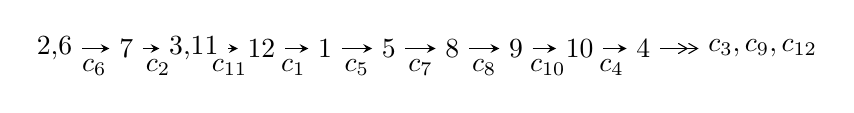
\begin{tikzpicture}[x=23pt, y=7pt]
	% node
	\node (A0) at (-1/8, 0) {2,6};
	\node (A1) at (1, 0) {7};
	\node (A2) at (33/16, 0) {3,11};
	\node (A3) at (25/8, 0) {12};
	\node (A4) at (33/8, 0) {1};
	\node (A5) at (41/8, 0) {5};
	\node (A6) at (49/8, 0) {8};
	\node (A7) at (57/8, 0) {9};
	\node (A8) at (65/8, 0) {10};
	\node (A9) at (73/8, 0) {4};
	\node (C1) at (1/2, -1) {$c_{6}$};
	\node (C2) at (3/2, -1) {$c_{2}$};
	\node (C3) at (21/8, -1) {$c_{11}$};
	\node (C4) at (29/8, -1) {$c_{1}$};
	\node (C5) at (37/8, -1) {$c_{5}$};
	\node (C6) at (45/8, -1) {$c_{7}$};
	\node (C7) at (53/8, -1) {$c_{8}$};
	\node (C8) at (61/8, -1) {$c_{10}$};
	\node (C9) at (69/8, -1) {$c_{4}$};
	\node (A10) at (11, 0) {$c_{3},c_{9},c_{12}$};

	% edge
	\draw[->,>=stealth]	
	(A0) edge (A1) (A1) edge (A2) (A2) edge (A3) (A3) edge (A4) (A4) edge (A5) (A5) edge (A6) (A6) edge (A7) (A7) edge (A8) (A8) edge (A9) ;
	\draw[->>,>={angle 60}]	
	(A9) edge (A10);
\end{tikzpicture} \\ 

\end{tabular} \\

\footnotetext{
The image of knot diagram is generated by the software ``\textbf{Draw programme}" developed by Andrew Bartholomew(\url{http://www.layer8.co.uk/maths/draw/index.htm\#Running-draw}), where we modified some parts for our purpose(\url{https://github.com/CATsTAILs/LinksPainter}).
}\phantom \\ \newline 
\centering \textbf{Ideals for irreducible components\footnotemark of $X_{\text{par}}$} 
 
\begin{align*}
I^u_{1}&=\langle 
3.95686\times10^{684} u^{182}-3.08751\times10^{684} u^{181}+\cdots+4.57143\times10^{684} b-1.11694\times10^{685},\\
\phantom{I^u_{1}}&\phantom{= \langle  }-3.33768\times10^{683} u^{182}+9.09273\times10^{683} u^{181}+\cdots+4.57143\times10^{684} a+1.34804\times10^{685},\\
\phantom{I^u_{1}}&\phantom{= \langle  }u^{183}- u^{182}+\cdots-26 u+1\rangle \\
I^u_{2}&=\langle 
-58996829294 u^{42}+102880855500 u^{41}+\cdots+11325634063 b-92288392095,\\
\phantom{I^u_{2}}&\phantom{= \langle  }-198008949584 u^{42}+286910003657 u^{41}+\cdots+11325634063 a-224634503866,\\
\phantom{I^u_{2}}&\phantom{= \langle  }u^{43}- u^{42}+\cdots+u+1\rangle \\
I^u_{3}&=\langle 
b,\;a-1,\;u+1\rangle \\
\\
\end{align*}
\raggedright * 3 irreducible components of $\dim_{\mathbb{C}}=0$, with total 227 representations.\\
\footnotetext{All coefficients of polynomials are rational numbers. But the coefficients are sometimes approximated in decimal forms when there is not enough margin.}
\newpage
\renewcommand{\arraystretch}{1}
\centering \section*{I. $I^u_{1}= \langle 3.96\times10^{684} u^{182}-3.09\times10^{684} u^{181}+\cdots+4.57\times10^{684} b-1.12\times10^{685},\;-3.34\times10^{683} u^{182}+9.09\times10^{683} u^{181}+\cdots+4.57\times10^{684} a+1.35\times10^{685},\;u^{183}- u^{182}+\cdots-26 u+1 \rangle$}
\flushleft \textbf{(i) Arc colorings}\\
\begin{tabular}{m{7pt} m{180pt} m{7pt} m{180pt} }
\flushright $a_{2}=$&$\begin{pmatrix}0\\u\end{pmatrix}$ \\
\flushright $a_{6}=$&$\begin{pmatrix}1\\0\end{pmatrix}$ \\
\flushright $a_{7}=$&$\begin{pmatrix}1\\u^2\end{pmatrix}$ \\
\flushright $a_{3}=$&$\begin{pmatrix}- u\\- u^3+u\end{pmatrix}$ \\
\flushright $a_{11}=$&$\begin{pmatrix}0.0730118 u^{182}-0.198904 u^{181}+\cdots+90.5142 u-2.94884\\-0.865563 u^{182}+0.675393 u^{181}+\cdots-82.7947 u+2.44331\end{pmatrix}$ \\
\flushright $a_{12}=$&$\begin{pmatrix}0.938575 u^{182}-0.874297 u^{181}+\cdots+173.309 u-5.39215\\-0.865563 u^{182}+0.675393 u^{181}+\cdots-82.7947 u+2.44331\end{pmatrix}$ \\
\flushright $a_{1}=$&$\begin{pmatrix}u^3\\u^5- u^3+u\end{pmatrix}$ \\
\flushright $a_{5}=$&$\begin{pmatrix}1.98433 u^{182}-1.70198 u^{181}+\cdots+256.368 u-7.59514\\-0.881093 u^{182}+0.671278 u^{181}+\cdots-69.2985 u+1.52425\end{pmatrix}$ \\
\flushright $a_{8}=$&$\begin{pmatrix}-1.97660 u^{182}+1.44326 u^{181}+\cdots-46.7057 u-5.66718\\-0.730808 u^{182}+0.708014 u^{181}+\cdots-163.139 u+9.24102\end{pmatrix}$ \\
\flushright $a_{9}=$&$\begin{pmatrix}-4.30363 u^{182}+3.58723 u^{181}+\cdots-503.736 u+16.0646\\-0.912461 u^{182}+0.810284 u^{181}+\cdots-164.734 u+10.5737\end{pmatrix}$ \\
\flushright $a_{10}=$&$\begin{pmatrix}-4.31508 u^{182}+3.59217 u^{181}+\cdots-504.738 u+16.1070\\-1.02164 u^{182}+0.890038 u^{181}+\cdots-177.623 u+11.2268\end{pmatrix}$ \\
\flushright $a_{4}=$&$\begin{pmatrix}-1.13902 u^{182}+0.855105 u^{181}+\cdots-104.038 u-2.14870\\0.627441 u^{182}-0.503619 u^{181}+\cdots+38.3100 u+0.604035\end{pmatrix}$\\&\end{tabular}
\flushleft \textbf{(ii) Obstruction class $= -1$}\\~\\
\flushleft \textbf{(iii) Cusp Shapes $= -1.55871 u^{182}+1.98436 u^{181}+\cdots-601.882 u+26.8946$}\\~\\
\newpage\renewcommand{\arraystretch}{1}
\flushleft \textbf{(iv) u-Polynomials at the component}\newline \\
\begin{tabular}{m{50pt}|m{274pt}}
Crossings & \hspace{64pt}u-Polynomials at each crossing \\
\hline $$\begin{aligned}c_{1}\end{aligned}$$&$\begin{aligned}
&u^{183}+73 u^{182}+\cdots+140 u+1
\end{aligned}$\\
\hline $$\begin{aligned}c_{2},c_{6}\end{aligned}$$&$\begin{aligned}
&u^{183}- u^{182}+\cdots-26 u+1
\end{aligned}$\\
\hline $$\begin{aligned}c_{3}\end{aligned}$$&$\begin{aligned}
&u^{183}+16 u^{181}+\cdots+13120 u-6587
\end{aligned}$\\
\hline $$\begin{aligned}c_{4}\end{aligned}$$&$\begin{aligned}
&u^{183}+3 u^{182}+\cdots+23844880676 u+2117995963
\end{aligned}$\\
\hline $$\begin{aligned}c_{5},c_{11}\end{aligned}$$&$\begin{aligned}
&u^{183}-59 u^{181}+\cdots+49924 u+6638
\end{aligned}$\\
\hline $$\begin{aligned}c_{7}\end{aligned}$$&$\begin{aligned}
&u^{183}-4 u^{182}+\cdots-79 u+1
\end{aligned}$\\
\hline $$\begin{aligned}c_{8}\end{aligned}$$&$\begin{aligned}
&u^{183}+u^{182}+\cdots-49629456462 u+10428858667
\end{aligned}$\\
\hline $$\begin{aligned}c_{9}\end{aligned}$$&$\begin{aligned}
&u^{183}+11 u^{182}+\cdots-25134 u+3142
\end{aligned}$\\
\hline $$\begin{aligned}c_{10}\end{aligned}$$&$\begin{aligned}
&u^{183}-7 u^{182}+\cdots-7 u-1
\end{aligned}$\\
\hline $$\begin{aligned}c_{12}\end{aligned}$$&$\begin{aligned}
&u^{183}+17 u^{182}+\cdots+3 u+1
\end{aligned}$\\
\hline
\end{tabular}\\~\\
\newpage\renewcommand{\arraystretch}{1}
\flushleft \textbf{(v) Riley Polynomials at the component}\newline \\
\begin{tabular}{m{50pt}|m{274pt}}
Crossings & \hspace{64pt}Riley Polynomials at each crossing \\
\hline $$\begin{aligned}c_{1}\end{aligned}$$&$\begin{aligned}
&y^{183}+71 y^{182}+\cdots-14140 y-1
\end{aligned}$\\
\hline $$\begin{aligned}c_{2},c_{6}\end{aligned}$$&$\begin{aligned}
&y^{183}-73 y^{182}+\cdots+140 y-1
\end{aligned}$\\
\hline $$\begin{aligned}c_{3}\end{aligned}$$&$\begin{aligned}
&y^{183}+32 y^{182}+\cdots-197765172 y-43388569
\end{aligned}$\\
\hline $$\begin{aligned}c_{4}\end{aligned}$$&$\begin{aligned}
&y^{183}-97 y^{182}+\cdots+5.30\times10^{20} y-4.49\times10^{18}
\end{aligned}$\\
\hline $$\begin{aligned}c_{5},c_{11}\end{aligned}$$&$\begin{aligned}
&y^{183}-118 y^{182}+\cdots+4475548104 y-44063044
\end{aligned}$\\
\hline $$\begin{aligned}c_{7}\end{aligned}$$&$\begin{aligned}
&y^{183}+4 y^{182}+\cdots+1331 y-1
\end{aligned}$\\
\hline $$\begin{aligned}c_{8}\end{aligned}$$&$\begin{aligned}
&y^{183}-73 y^{182}+\cdots+3.70\times10^{21} y-1.09\times10^{20}
\end{aligned}$\\
\hline $$\begin{aligned}c_{9}\end{aligned}$$&$\begin{aligned}
&y^{183}+47 y^{182}+\cdots+8565230252 y-9872164
\end{aligned}$\\
\hline $$\begin{aligned}c_{10}\end{aligned}$$&$\begin{aligned}
&y^{183}-17 y^{182}+\cdots+23 y-1
\end{aligned}$\\
\hline $$\begin{aligned}c_{12}\end{aligned}$$&$\begin{aligned}
&y^{183}-49 y^{182}+\cdots-71 y-1
\end{aligned}$\\
\hline
\end{tabular}\\~\\
\newpage\flushleft \textbf{(vi) Complex Volumes and Cusp Shapes}
$$\begin{array}{c|c|c}  
\text{Solutions to }I^u_{1}& \I (\text{vol} + \sqrt{-1}CS) & \text{Cusp shape}\\
 \hline 
\begin{aligned}
u &= -0.804086 + 0.597313 I \\
a &= -1.88182 - 1.85240 I \\
b &= -1.51604 + 0.72956 I\end{aligned}
 & \phantom{-}0.78321 + 5.97914 I & \phantom{-0.000000 } 0 \\ \hline\begin{aligned}
u &= -0.804086 - 0.597313 I \\
a &= -1.88182 + 1.85240 I \\
b &= -1.51604 - 0.72956 I\end{aligned}
 & \phantom{-}0.78321 - 5.97914 I & \phantom{-0.000000 } 0 \\ \hline\begin{aligned}
u &= -0.968465 + 0.204179 I \\
a &= \phantom{-}0.681431 - 0.690236 I \\
b &= \phantom{-}0.254549 - 1.090810 I\end{aligned}
 & -2.78855 + 0.17947 I & \phantom{-0.000000 } 0 \\ \hline\begin{aligned}
u &= -0.968465 - 0.204179 I \\
a &= \phantom{-}0.681431 + 0.690236 I \\
b &= \phantom{-}0.254549 + 1.090810 I\end{aligned}
 & -2.78855 - 0.17947 I & \phantom{-0.000000 } 0 \\ \hline\begin{aligned}
u &= \phantom{-}0.784543 + 0.583880 I \\
a &= -1.35379 + 1.73904 I \\
b &= -0.967185 - 0.955823 I\end{aligned}
 & -0.075537 + 0.190930 I & \phantom{-0.000000 } 0 \\ \hline\begin{aligned}
u &= \phantom{-}0.784543 - 0.583880 I \\
a &= -1.35379 - 1.73904 I \\
b &= -0.967185 + 0.955823 I\end{aligned}
 & -0.075537 - 0.190930 I & \phantom{-0.000000 } 0 \\ \hline\begin{aligned}
u &= \phantom{-}0.771537 + 0.677709 I \\
a &= -0.219574 + 0.755952 I \\
b &= -0.471848 - 0.886299 I\end{aligned}
 & \phantom{-}4.28626 + 0.70719 I & \phantom{-0.000000 } 0 \\ \hline\begin{aligned}
u &= \phantom{-}0.771537 - 0.677709 I \\
a &= -0.219574 - 0.755952 I \\
b &= -0.471848 + 0.886299 I\end{aligned}
 & \phantom{-}4.28626 - 0.70719 I & \phantom{-0.000000 } 0 \\ \hline\begin{aligned}
u &= -0.615624 + 0.744589 I \\
a &= \phantom{-}0.206463 + 0.385144 I \\
b &= -1.158630 - 0.701322 I\end{aligned}
 & -1.26582 - 6.65398 I & \phantom{-0.000000 } 0 \\ \hline\begin{aligned}
u &= -0.615624 - 0.744589 I \\
a &= \phantom{-}0.206463 - 0.385144 I \\
b &= -1.158630 + 0.701322 I\end{aligned}
 & -1.26582 + 6.65398 I & \phantom{-0.000000 } 0\\
 \hline 
 \end{array}$$\newpage$$\begin{array}{c|c|c}  
\text{Solutions to }I^u_{1}& \I (\text{vol} + \sqrt{-1}CS) & \text{Cusp shape}\\
 \hline 
\begin{aligned}
u &= \phantom{-}0.945595 + 0.185636 I \\
a &= -0.374523 - 0.991767 I \\
b &= \phantom{-}0.192487 + 0.021372 I\end{aligned}
 & -2.72218 - 3.83344 I & \phantom{-0.000000 } 0 \\ \hline\begin{aligned}
u &= \phantom{-}0.945595 - 0.185636 I \\
a &= -0.374523 + 0.991767 I \\
b &= \phantom{-}0.192487 - 0.021372 I\end{aligned}
 & -2.72218 + 3.83344 I & \phantom{-0.000000 } 0 \\ \hline\begin{aligned}
u &= \phantom{-}0.957428 + 0.082830 I \\
a &= \phantom{-}1.35226 - 1.44806 I \\
b &= \phantom{-}1.090440 + 0.388673 I\end{aligned}
 & -2.41546 - 5.59132 I & \phantom{-0.000000 } 0 \\ \hline\begin{aligned}
u &= \phantom{-}0.957428 - 0.082830 I \\
a &= \phantom{-}1.35226 + 1.44806 I \\
b &= \phantom{-}1.090440 - 0.388673 I\end{aligned}
 & -2.41546 + 5.59132 I & \phantom{-0.000000 } 0 \\ \hline\begin{aligned}
u &= \phantom{-}1.044680 + 0.083571 I \\
a &= \phantom{-}2.64047 - 0.64175 I \\
b &= \phantom{-}1.085590 - 0.408152 I\end{aligned}
 & -2.41862 + 5.61416 I & \phantom{-0.000000 } 0 \\ \hline\begin{aligned}
u &= \phantom{-}1.044680 - 0.083571 I \\
a &= \phantom{-}2.64047 + 0.64175 I \\
b &= \phantom{-}1.085590 + 0.408152 I\end{aligned}
 & -2.41862 - 5.61416 I & \phantom{-0.000000 } 0 \\ \hline\begin{aligned}
u &= -0.659362 + 0.686197 I \\
a &= -0.448274 + 0.614066 I \\
b &= -1.130220 - 0.617602 I\end{aligned}
 & \phantom{-}2.20599 - 6.27476 I & \phantom{-0.000000 } 0 \\ \hline\begin{aligned}
u &= -0.659362 - 0.686197 I \\
a &= -0.448274 - 0.614066 I \\
b &= -1.130220 + 0.617602 I\end{aligned}
 & \phantom{-}2.20599 + 6.27476 I & \phantom{-0.000000 } 0 \\ \hline\begin{aligned}
u &= \phantom{-}0.667868 + 0.659329 I \\
a &= -1.401060 - 0.059418 I \\
b &= -1.269760 + 0.374151 I\end{aligned}
 & -1.39366 + 5.27272 I & \phantom{-0.000000 } 0 \\ \hline\begin{aligned}
u &= \phantom{-}0.667868 - 0.659329 I \\
a &= -1.401060 + 0.059418 I \\
b &= -1.269760 - 0.374151 I\end{aligned}
 & -1.39366 - 5.27272 I & \phantom{-0.000000 } 0\\
 \hline 
 \end{array}$$\newpage$$\begin{array}{c|c|c}  
\text{Solutions to }I^u_{1}& \I (\text{vol} + \sqrt{-1}CS) & \text{Cusp shape}\\
 \hline 
\begin{aligned}
u &= -0.832572 + 0.659769 I \\
a &= -0.798710 - 0.102024 I \\
b &= -0.127155 + 1.264060 I\end{aligned}
 & \phantom{-}5.11906 + 0.42514 I & \phantom{-0.000000 } 0 \\ \hline\begin{aligned}
u &= -0.832572 - 0.659769 I \\
a &= -0.798710 + 0.102024 I \\
b &= -0.127155 - 1.264060 I\end{aligned}
 & \phantom{-}5.11906 - 0.42514 I & \phantom{-0.000000 } 0 \\ \hline\begin{aligned}
u &= -0.721508 + 0.781473 I \\
a &= \phantom{-}1.150080 + 0.773882 I \\
b &= -0.913552 - 0.200853 I\end{aligned}
 & \phantom{-}3.37130 - 4.99253 I & \phantom{-0.000000 } 0 \\ \hline\begin{aligned}
u &= -0.721508 - 0.781473 I \\
a &= \phantom{-}1.150080 - 0.773882 I \\
b &= -0.913552 + 0.200853 I\end{aligned}
 & \phantom{-}3.37130 + 4.99253 I & \phantom{-0.000000 } 0 \\ \hline\begin{aligned}
u &= -1.061230 + 0.074993 I \\
a &= \phantom{-}2.81778 + 1.07027 I \\
b &= \phantom{-}1.193020 + 0.134541 I\end{aligned}
 & -5.88372 - 4.47978 I & \phantom{-0.000000 } 0 \\ \hline\begin{aligned}
u &= -1.061230 - 0.074993 I \\
a &= \phantom{-}2.81778 - 1.07027 I \\
b &= \phantom{-}1.193020 - 0.134541 I\end{aligned}
 & -5.88372 + 4.47978 I & \phantom{-0.000000 } 0 \\ \hline\begin{aligned}
u &= \phantom{-}0.729768 + 0.580809 I \\
a &= -2.01374 + 3.77134 I \\
b &= -0.875001 - 0.160538 I\end{aligned}
 & \phantom{-}3.59621 + 3.18555 I & \phantom{-0.000000 } 0 \\ \hline\begin{aligned}
u &= \phantom{-}0.729768 - 0.580809 I \\
a &= -2.01374 - 3.77134 I \\
b &= -0.875001 + 0.160538 I\end{aligned}
 & \phantom{-}3.59621 - 3.18555 I & \phantom{-0.000000 } 0 \\ \hline\begin{aligned}
u &= \phantom{-}0.775056 + 0.741065 I \\
a &= \phantom{-}0.468878 + 0.589716 I \\
b &= -0.574447 - 0.328403 I\end{aligned}
 & \phantom{-}4.07080 - 1.71524 I & \phantom{-0.000000 } 0 \\ \hline\begin{aligned}
u &= \phantom{-}0.775056 - 0.741065 I \\
a &= \phantom{-}0.468878 - 0.589716 I \\
b &= -0.574447 + 0.328403 I\end{aligned}
 & \phantom{-}4.07080 + 1.71524 I & \phantom{-0.000000 } 0\\
 \hline 
 \end{array}$$\newpage$$\begin{array}{c|c|c}  
\text{Solutions to }I^u_{1}& \I (\text{vol} + \sqrt{-1}CS) & \text{Cusp shape}\\
 \hline 
\begin{aligned}
u &= \phantom{-}0.855253 + 0.647139 I \\
a &= \phantom{-}0.734078 - 0.607230 I \\
b &= \phantom{-}0.095770 + 0.753563 I\end{aligned}
 & \phantom{-}2.37109 - 2.52576 I & \phantom{-0.000000 } 0 \\ \hline\begin{aligned}
u &= \phantom{-}0.855253 - 0.647139 I \\
a &= \phantom{-}0.734078 + 0.607230 I \\
b &= \phantom{-}0.095770 - 0.753563 I\end{aligned}
 & \phantom{-}2.37109 + 2.52576 I & \phantom{-0.000000 } 0 \\ \hline\begin{aligned}
u &= -0.890607 + 0.602506 I \\
a &= \phantom{-}0.257989 + 0.377581 I \\
b &= \phantom{-}1.27916 + 0.78291 I\end{aligned}
 & \phantom{-}0.491769 - 1.227750 I & \phantom{-0.000000 } 0 \\ \hline\begin{aligned}
u &= -0.890607 - 0.602506 I \\
a &= \phantom{-}0.257989 - 0.377581 I \\
b &= \phantom{-}1.27916 - 0.78291 I\end{aligned}
 & \phantom{-}0.491769 + 1.227750 I & \phantom{-0.000000 } 0 \\ \hline\begin{aligned}
u &= -1.073610 + 0.089757 I \\
a &= \phantom{-}2.26071 + 0.88250 I \\
b &= \phantom{-}1.275060 + 0.359848 I\end{aligned}
 & -3.01048 - 5.23037 I & \phantom{-0.000000 } 0 \\ \hline\begin{aligned}
u &= -1.073610 - 0.089757 I \\
a &= \phantom{-}2.26071 - 0.88250 I \\
b &= \phantom{-}1.275060 - 0.359848 I\end{aligned}
 & -3.01048 + 5.23037 I & \phantom{-0.000000 } 0 \\ \hline\begin{aligned}
u &= -0.650827 + 0.646025 I \\
a &= -1.10330 + 1.14170 I \\
b &= -0.906991 - 0.382241 I\end{aligned}
 & \phantom{-}3.12157 - 1.56300 I & \phantom{-0.000000 } 0 \\ \hline\begin{aligned}
u &= -0.650827 - 0.646025 I \\
a &= -1.10330 - 1.14170 I \\
b &= -0.906991 + 0.382241 I\end{aligned}
 & \phantom{-}3.12157 + 1.56300 I & \phantom{-0.000000 } 0 \\ \hline\begin{aligned}
u &= -0.579718 + 0.707338 I \\
a &= \phantom{-}0.440010 - 0.100121 I \\
b &= \phantom{-}1.171120 + 0.371476 I\end{aligned}
 & -1.07062 - 1.30229 I & \phantom{-0.000000 } 0 \\ \hline\begin{aligned}
u &= -0.579718 - 0.707338 I \\
a &= \phantom{-}0.440010 + 0.100121 I \\
b &= \phantom{-}1.171120 - 0.371476 I\end{aligned}
 & -1.07062 + 1.30229 I & \phantom{-0.000000 } 0\\
 \hline 
 \end{array}$$\newpage$$\begin{array}{c|c|c}  
\text{Solutions to }I^u_{1}& \I (\text{vol} + \sqrt{-1}CS) & \text{Cusp shape}\\
 \hline 
\begin{aligned}
u &= -0.627576 + 0.889503 I \\
a &= \phantom{-}0.613731 + 0.583837 I \\
b &= \phantom{-}0.201181 - 1.124280 I\end{aligned}
 & \phantom{-}6.86968 - 8.72601 I & \phantom{-0.000000 } 0 \\ \hline\begin{aligned}
u &= -0.627576 - 0.889503 I \\
a &= \phantom{-}0.613731 - 0.583837 I \\
b &= \phantom{-}0.201181 + 1.124280 I\end{aligned}
 & \phantom{-}6.86968 + 8.72601 I & \phantom{-0.000000 } 0 \\ \hline\begin{aligned}
u &= \phantom{-}1.089170 + 0.004309 I \\
a &= \phantom{-}2.29605 - 0.19777 I \\
b &= \phantom{-}1.34165 - 0.51669 I\end{aligned}
 & -6.71040 + 5.77636 I & \phantom{-0.000000 } 0 \\ \hline\begin{aligned}
u &= \phantom{-}1.089170 - 0.004309 I \\
a &= \phantom{-}2.29605 + 0.19777 I \\
b &= \phantom{-}1.34165 + 0.51669 I\end{aligned}
 & -6.71040 - 5.77636 I & \phantom{-0.000000 } 0 \\ \hline\begin{aligned}
u &= -0.845242 + 0.688470 I \\
a &= \phantom{-}0.272507 - 0.178473 I \\
b &= \phantom{-}0.868210 + 0.212625 I\end{aligned}
 & -0.668854 + 0.328108 I & \phantom{-0.000000 } 0 \\ \hline\begin{aligned}
u &= -0.845242 - 0.688470 I \\
a &= \phantom{-}0.272507 + 0.178473 I \\
b &= \phantom{-}0.868210 - 0.212625 I\end{aligned}
 & -0.668854 - 0.328108 I & \phantom{-0.000000 } 0 \\ \hline\begin{aligned}
u &= -0.871720 + 0.659803 I \\
a &= -1.149790 + 0.097355 I \\
b &= -0.079998 + 1.289210 I\end{aligned}
 & \phantom{-}4.99782 + 4.69561 I & \phantom{-0.000000 } 0 \\ \hline\begin{aligned}
u &= -0.871720 - 0.659803 I \\
a &= -1.149790 - 0.097355 I \\
b &= -0.079998 - 1.289210 I\end{aligned}
 & \phantom{-}4.99782 - 4.69561 I & \phantom{-0.000000 } 0 \\ \hline\begin{aligned}
u &= -0.904516 + 0.053439 I \\
a &= \phantom{-}0.640466 + 1.121410 I \\
b &= \phantom{-}0.389672 + 0.665385 I\end{aligned}
 & -0.28611 + 1.59809 I & \phantom{-0.000000 } 0 \\ \hline\begin{aligned}
u &= -0.904516 - 0.053439 I \\
a &= \phantom{-}0.640466 - 1.121410 I \\
b &= \phantom{-}0.389672 - 0.665385 I\end{aligned}
 & -0.28611 - 1.59809 I & \phantom{-0.000000 } 0\\
 \hline 
 \end{array}$$\newpage$$\begin{array}{c|c|c}  
\text{Solutions to }I^u_{1}& \I (\text{vol} + \sqrt{-1}CS) & \text{Cusp shape}\\
 \hline 
\begin{aligned}
u &= \phantom{-}0.622313 + 0.653580 I \\
a &= -0.305034 + 0.132693 I \\
b &= -1.28668 + 0.68962 I\end{aligned}
 & \phantom{-}1.57573 + 6.31832 I & \phantom{-0.000000 } 0 \\ \hline\begin{aligned}
u &= \phantom{-}0.622313 - 0.653580 I \\
a &= -0.305034 - 0.132693 I \\
b &= -1.28668 - 0.68962 I\end{aligned}
 & \phantom{-}1.57573 - 6.31832 I & \phantom{-0.000000 } 0 \\ \hline\begin{aligned}
u &= -0.836262 + 0.715392 I \\
a &= -0.881213 - 0.326547 I \\
b &= -0.610782 + 0.802006 I\end{aligned}
 & \phantom{-}3.47032 + 6.94246 I & \phantom{-0.000000 } 0 \\ \hline\begin{aligned}
u &= -0.836262 - 0.715392 I \\
a &= -0.881213 + 0.326547 I \\
b &= -0.610782 - 0.802006 I\end{aligned}
 & \phantom{-}3.47032 - 6.94246 I & \phantom{-0.000000 } 0 \\ \hline\begin{aligned}
u &= \phantom{-}0.581389 + 0.936165 I \\
a &= \phantom{-}0.646479 - 0.595519 I \\
b &= \phantom{-}0.167723 + 1.025120 I\end{aligned}
 & \phantom{-}6.68101 + 0.05061 I & \phantom{-0.000000 } 0 \\ \hline\begin{aligned}
u &= \phantom{-}0.581389 - 0.936165 I \\
a &= \phantom{-}0.646479 + 0.595519 I \\
b &= \phantom{-}0.167723 - 1.025120 I\end{aligned}
 & \phantom{-}6.68101 - 0.05061 I & \phantom{-0.000000 } 0 \\ \hline\begin{aligned}
u &= \phantom{-}0.931243 + 0.599868 I \\
a &= -0.682656 - 0.275411 I \\
b &= \phantom{-}0.808521 - 1.117020 I\end{aligned}
 & -0.56324 - 4.88976 I & \phantom{-0.000000 } 0 \\ \hline\begin{aligned}
u &= \phantom{-}0.931243 - 0.599868 I \\
a &= -0.682656 + 0.275411 I \\
b &= \phantom{-}0.808521 + 1.117020 I\end{aligned}
 & -0.56324 + 4.88976 I & \phantom{-0.000000 } 0 \\ \hline\begin{aligned}
u &= \phantom{-}1.107390 + 0.045773 I \\
a &= -2.49976 + 0.23421 I \\
b &= -1.259940 + 0.064021 I\end{aligned}
 & -6.26958 + 0.10015 I & \phantom{-0.000000 } 0 \\ \hline\begin{aligned}
u &= \phantom{-}1.107390 - 0.045773 I \\
a &= -2.49976 - 0.23421 I \\
b &= -1.259940 - 0.064021 I\end{aligned}
 & -6.26958 - 0.10015 I & \phantom{-0.000000 } 0\\
 \hline 
 \end{array}$$\newpage$$\begin{array}{c|c|c}  
\text{Solutions to }I^u_{1}& \I (\text{vol} + \sqrt{-1}CS) & \text{Cusp shape}\\
 \hline 
\begin{aligned}
u &= \phantom{-}0.774080 + 0.797223 I \\
a &= \phantom{-}0.897507 - 0.250365 I \\
b &= -0.588803 + 0.436380 I\end{aligned}
 & \phantom{-}3.87932 - 2.29960 I & \phantom{-0.000000 } 0 \\ \hline\begin{aligned}
u &= \phantom{-}0.774080 - 0.797223 I \\
a &= \phantom{-}0.897507 + 0.250365 I \\
b &= -0.588803 - 0.436380 I\end{aligned}
 & \phantom{-}3.87932 + 2.29960 I & \phantom{-0.000000 } 0 \\ \hline\begin{aligned}
u &= -0.684988 + 0.565576 I \\
a &= -1.217240 + 0.438700 I \\
b &= -0.768663 - 0.508050 I\end{aligned}
 & \phantom{-}3.54233 + 2.09873 I & \phantom{-0.000000 } 0 \\ \hline\begin{aligned}
u &= -0.684988 - 0.565576 I \\
a &= -1.217240 - 0.438700 I \\
b &= -0.768663 + 0.508050 I\end{aligned}
 & \phantom{-}3.54233 - 2.09873 I & \phantom{-0.000000 } 0 \\ \hline\begin{aligned}
u &= \phantom{-}0.786078 + 0.787473 I \\
a &= -0.078362 + 0.381478 I \\
b &= -0.854273 - 0.355693 I\end{aligned}
 & \phantom{-}3.35990 - 5.71800 I & \phantom{-0.000000 } 0 \\ \hline\begin{aligned}
u &= \phantom{-}0.786078 - 0.787473 I \\
a &= -0.078362 - 0.381478 I \\
b &= -0.854273 + 0.355693 I\end{aligned}
 & \phantom{-}3.35990 + 5.71800 I & \phantom{-0.000000 } 0 \\ \hline\begin{aligned}
u &= -0.690384 + 0.549588 I \\
a &= -2.12381 - 4.03693 I \\
b &= -0.894453 + 0.251188 I\end{aligned}
 & \phantom{-}3.35823 + 5.37464 I & \phantom{-0.000000 } 0 \\ \hline\begin{aligned}
u &= -0.690384 - 0.549588 I \\
a &= -2.12381 + 4.03693 I \\
b &= -0.894453 - 0.251188 I\end{aligned}
 & \phantom{-}3.35823 - 5.37464 I & \phantom{-0.000000 } 0 \\ \hline\begin{aligned}
u &= -0.859618 + 0.716217 I \\
a &= -0.089129 + 0.288175 I \\
b &= \phantom{-}0.370265 + 0.757502 I\end{aligned}
 & \phantom{-}3.39992 - 1.47988 I & \phantom{-0.000000 } 0 \\ \hline\begin{aligned}
u &= -0.859618 - 0.716217 I \\
a &= -0.089129 - 0.288175 I \\
b &= \phantom{-}0.370265 - 0.757502 I\end{aligned}
 & \phantom{-}3.39992 + 1.47988 I & \phantom{-0.000000 } 0\\
 \hline 
 \end{array}$$\newpage$$\begin{array}{c|c|c}  
\text{Solutions to }I^u_{1}& \I (\text{vol} + \sqrt{-1}CS) & \text{Cusp shape}\\
 \hline 
\begin{aligned}
u &= -0.075302 + 0.868974 I \\
a &= \phantom{-}1.365680 - 0.359231 I \\
b &= \phantom{-}0.050464 + 0.310642 I\end{aligned}
 & \phantom{-}4.27203 + 4.69198 I & \phantom{-0.000000 } 0 \\ \hline\begin{aligned}
u &= -0.075302 - 0.868974 I \\
a &= \phantom{-}1.365680 + 0.359231 I \\
b &= \phantom{-}0.050464 - 0.310642 I\end{aligned}
 & \phantom{-}4.27203 - 4.69198 I & \phantom{-0.000000 } 0 \\ \hline\begin{aligned}
u &= -0.727939 + 0.461758 I \\
a &= -1.50335 - 1.58092 I \\
b &= -1.130880 - 0.380737 I\end{aligned}
 & -0.72886 + 2.94415 I & \phantom{-0.000000 } 0 \\ \hline\begin{aligned}
u &= -0.727939 - 0.461758 I \\
a &= -1.50335 + 1.58092 I \\
b &= -1.130880 + 0.380737 I\end{aligned}
 & -0.72886 - 2.94415 I & \phantom{-0.000000 } 0 \\ \hline\begin{aligned}
u &= \phantom{-}0.639216 + 0.570367 I \\
a &= -0.115708 - 0.172824 I \\
b &= -0.669171 + 0.759190 I\end{aligned}
 & \phantom{-}3.35772 - 1.25907 I & \phantom{-0.000000 } 0 \\ \hline\begin{aligned}
u &= \phantom{-}0.639216 - 0.570367 I \\
a &= -0.115708 + 0.172824 I \\
b &= -0.669171 - 0.759190 I\end{aligned}
 & \phantom{-}3.35772 + 1.25907 I & \phantom{-0.000000 } 0 \\ \hline\begin{aligned}
u &= -1.146440 + 0.063129 I \\
a &= -0.308983 + 0.148588 I \\
b &= \phantom{-}0.308825 - 0.627728 I\end{aligned}
 & -0.19824 - 1.63291 I & \phantom{-0.000000 } 0 \\ \hline\begin{aligned}
u &= -1.146440 - 0.063129 I \\
a &= -0.308983 - 0.148588 I \\
b &= \phantom{-}0.308825 + 0.627728 I\end{aligned}
 & -0.19824 + 1.63291 I & \phantom{-0.000000 } 0 \\ \hline\begin{aligned}
u &= \phantom{-}0.927993 + 0.676423 I \\
a &= -0.960077 - 0.279359 I \\
b &= \phantom{-}0.363758 - 0.892240 I\end{aligned}
 & \phantom{-}3.80950 - 5.94710 I & \phantom{-0.000000 } 0 \\ \hline\begin{aligned}
u &= \phantom{-}0.927993 - 0.676423 I \\
a &= -0.960077 + 0.279359 I \\
b &= \phantom{-}0.363758 + 0.892240 I\end{aligned}
 & \phantom{-}3.80950 + 5.94710 I & \phantom{-0.000000 } 0\\
 \hline 
 \end{array}$$\newpage$$\begin{array}{c|c|c}  
\text{Solutions to }I^u_{1}& \I (\text{vol} + \sqrt{-1}CS) & \text{Cusp shape}\\
 \hline 
\begin{aligned}
u &= \phantom{-}0.686652 + 0.500534 I \\
a &= -0.95150 + 2.41807 I \\
b &= -1.81120 + 0.22305 I\end{aligned}
 & -0.08217 + 3.42918 I & \phantom{-0.000000 } 0 \\ \hline\begin{aligned}
u &= \phantom{-}0.686652 - 0.500534 I \\
a &= -0.95150 - 2.41807 I \\
b &= -1.81120 - 0.22305 I\end{aligned}
 & -0.08217 - 3.42918 I & \phantom{-0.000000 } 0 \\ \hline\begin{aligned}
u &= \phantom{-}0.975940 + 0.609702 I \\
a &= \phantom{-}0.207008 + 1.318360 I \\
b &= \phantom{-}0.789006 - 0.337870 I\end{aligned}
 & \phantom{-}2.78038 - 7.93575 I & \phantom{-0.000000 } 0 \\ \hline\begin{aligned}
u &= \phantom{-}0.975940 - 0.609702 I \\
a &= \phantom{-}0.207008 - 1.318360 I \\
b &= \phantom{-}0.789006 + 0.337870 I\end{aligned}
 & \phantom{-}2.78038 + 7.93575 I & \phantom{-0.000000 } 0 \\ \hline\begin{aligned}
u &= -0.823980 + 0.807894 I \\
a &= -0.661366 - 1.182780 I \\
b &= -1.074960 + 0.309302 I\end{aligned}
 & -0.68075 + 5.27880 I & \phantom{-0.000000 } 0 \\ \hline\begin{aligned}
u &= -0.823980 - 0.807894 I \\
a &= -0.661366 + 1.182780 I \\
b &= -1.074960 - 0.309302 I\end{aligned}
 & -0.68075 - 5.27880 I & \phantom{-0.000000 } 0 \\ \hline\begin{aligned}
u &= -1.139910 + 0.213951 I \\
a &= \phantom{-}1.91706 + 0.32380 I \\
b &= \phantom{-}1.66770 - 0.79542 I\end{aligned}
 & -3.55957 - 1.18556 I & \phantom{-0.000000 } 0 \\ \hline\begin{aligned}
u &= -1.139910 - 0.213951 I \\
a &= \phantom{-}1.91706 - 0.32380 I \\
b &= \phantom{-}1.66770 + 0.79542 I\end{aligned}
 & -3.55957 + 1.18556 I & \phantom{-0.000000 } 0 \\ \hline\begin{aligned}
u &= \phantom{-}1.013210 + 0.568393 I \\
a &= \phantom{-}1.62756 - 0.95953 I \\
b &= \phantom{-}0.830652 + 0.499639 I\end{aligned}
 & \phantom{-}2.20875 - 3.36417 I & \phantom{-0.000000 } 0 \\ \hline\begin{aligned}
u &= \phantom{-}1.013210 - 0.568393 I \\
a &= \phantom{-}1.62756 + 0.95953 I \\
b &= \phantom{-}0.830652 - 0.499639 I\end{aligned}
 & \phantom{-}2.20875 + 3.36417 I & \phantom{-0.000000 } 0\\
 \hline 
 \end{array}$$\newpage$$\begin{array}{c|c|c}  
\text{Solutions to }I^u_{1}& \I (\text{vol} + \sqrt{-1}CS) & \text{Cusp shape}\\
 \hline 
\begin{aligned}
u &= \phantom{-}1.151840 + 0.154662 I \\
a &= \phantom{-}0.010016 + 0.398685 I \\
b &= \phantom{-}0.209573 + 0.978495 I\end{aligned}
 & -0.26884 - 7.85265 I & \phantom{-0.000000 } 0 \\ \hline\begin{aligned}
u &= \phantom{-}1.151840 - 0.154662 I \\
a &= \phantom{-}0.010016 - 0.398685 I \\
b &= \phantom{-}0.209573 - 0.978495 I\end{aligned}
 & -0.26884 + 7.85265 I & \phantom{-0.000000 } 0 \\ \hline\begin{aligned}
u &= -1.009310 + 0.577692 I \\
a &= \phantom{-}2.07833 + 0.93833 I \\
b &= \phantom{-}0.890024 - 0.287554 I\end{aligned}
 & \phantom{-}2.49438 + 2.50944 I & \phantom{-0.000000 } 0 \\ \hline\begin{aligned}
u &= -1.009310 - 0.577692 I \\
a &= \phantom{-}2.07833 - 0.93833 I \\
b &= \phantom{-}0.890024 + 0.287554 I\end{aligned}
 & \phantom{-}2.49438 - 2.50944 I & \phantom{-0.000000 } 0 \\ \hline\begin{aligned}
u &= \phantom{-}1.010010 + 0.582201 I \\
a &= \phantom{-}1.26803 - 1.31464 I \\
b &= \phantom{-}1.97259 - 0.08099 I\end{aligned}
 & -1.22638 - 7.91000 I & \phantom{-0.000000 } 0 \\ \hline\begin{aligned}
u &= \phantom{-}1.010010 - 0.582201 I \\
a &= \phantom{-}1.26803 + 1.31464 I \\
b &= \phantom{-}1.97259 + 0.08099 I\end{aligned}
 & -1.22638 + 7.91000 I & \phantom{-0.000000 } 0 \\ \hline\begin{aligned}
u &= \phantom{-}0.602125 + 1.010350 I \\
a &= \phantom{-}0.436257 + 0.244031 I \\
b &= \phantom{-}1.28843 - 0.60858 I\end{aligned}
 & \phantom{-}3.4487 + 14.8188 I & \phantom{-0.000000 } 0 \\ \hline\begin{aligned}
u &= \phantom{-}0.602125 - 1.010350 I \\
a &= \phantom{-}0.436257 - 0.244031 I \\
b &= \phantom{-}1.28843 + 0.60858 I\end{aligned}
 & \phantom{-}3.4487 - 14.8188 I & \phantom{-0.000000 } 0 \\ \hline\begin{aligned}
u &= \phantom{-}1.18146\phantom{ +0.000000I} \\
a &= \phantom{-}2.68363\phantom{ +0.000000I} \\
b &= \phantom{-}0.963202\phantom{ +0.000000I}\end{aligned}
 & -1.54825\phantom{ +0.000000I} & \phantom{-0.000000 } 0 \\ \hline\begin{aligned}
u &= \phantom{-}0.942284 + 0.716877 I \\
a &= -0.666318 - 0.369851 I \\
b &= \phantom{-}0.520947 - 0.232184 I\end{aligned}
 & \phantom{-}3.56771 - 3.83933 I & \phantom{-0.000000 } 0\\
 \hline 
 \end{array}$$\newpage$$\begin{array}{c|c|c}  
\text{Solutions to }I^u_{1}& \I (\text{vol} + \sqrt{-1}CS) & \text{Cusp shape}\\
 \hline 
\begin{aligned}
u &= \phantom{-}0.942284 - 0.716877 I \\
a &= -0.666318 + 0.369851 I \\
b &= \phantom{-}0.520947 + 0.232184 I\end{aligned}
 & \phantom{-}3.56771 + 3.83933 I & \phantom{-0.000000 } 0 \\ \hline\begin{aligned}
u &= \phantom{-}0.994283 + 0.644562 I \\
a &= \phantom{-}2.27949 - 1.45447 I \\
b &= \phantom{-}1.334210 + 0.319655 I\end{aligned}
 & -2.38828 - 10.38320 I & \phantom{-0.000000 } 0 \\ \hline\begin{aligned}
u &= \phantom{-}0.994283 - 0.644562 I \\
a &= \phantom{-}2.27949 + 1.45447 I \\
b &= \phantom{-}1.334210 - 0.319655 I\end{aligned}
 & -2.38828 + 10.38320 I & \phantom{-0.000000 } 0 \\ \hline\begin{aligned}
u &= \phantom{-}0.474515 + 0.656195 I \\
a &= \phantom{-}0.406059 + 0.098625 I \\
b &= -1.079700 + 0.698453 I\end{aligned}
 & \phantom{-}1.91142 + 2.58746 I & \phantom{-0.000000 } 0 \\ \hline\begin{aligned}
u &= \phantom{-}0.474515 - 0.656195 I \\
a &= \phantom{-}0.406059 - 0.098625 I \\
b &= -1.079700 - 0.698453 I\end{aligned}
 & \phantom{-}1.91142 - 2.58746 I & \phantom{-0.000000 } 0 \\ \hline\begin{aligned}
u &= -1.008370 + 0.638657 I \\
a &= \phantom{-}2.12903 + 1.73560 I \\
b &= \phantom{-}1.018580 - 0.326923 I\end{aligned}
 & \phantom{-}2.02276 + 6.62718 I & \phantom{-0.000000 } 0 \\ \hline\begin{aligned}
u &= -1.008370 - 0.638657 I \\
a &= \phantom{-}2.12903 - 1.73560 I \\
b &= \phantom{-}1.018580 + 0.326923 I\end{aligned}
 & \phantom{-}2.02276 - 6.62718 I & \phantom{-0.000000 } 0 \\ \hline\begin{aligned}
u &= \phantom{-}1.009840 + 0.636828 I \\
a &= \phantom{-}1.95063 - 1.37133 I \\
b &= \phantom{-}1.41880 + 0.63898 I\end{aligned}
 & \phantom{-}0.41909 - 11.39740 I & \phantom{-0.000000 } 0 \\ \hline\begin{aligned}
u &= \phantom{-}1.009840 - 0.636828 I \\
a &= \phantom{-}1.95063 + 1.37133 I \\
b &= \phantom{-}1.41880 - 0.63898 I\end{aligned}
 & \phantom{-}0.41909 + 11.39740 I & \phantom{-0.000000 } 0 \\ \hline\begin{aligned}
u &= -1.000030 + 0.652330 I \\
a &= \phantom{-}1.95082 + 1.70847 I \\
b &= \phantom{-}1.201080 - 0.593735 I\end{aligned}
 & \phantom{-}1.17604 + 11.47750 I & \phantom{-0.000000 } 0\\
 \hline 
 \end{array}$$\newpage$$\begin{array}{c|c|c}  
\text{Solutions to }I^u_{1}& \I (\text{vol} + \sqrt{-1}CS) & \text{Cusp shape}\\
 \hline 
\begin{aligned}
u &= -1.000030 - 0.652330 I \\
a &= \phantom{-}1.95082 - 1.70847 I \\
b &= \phantom{-}1.201080 + 0.593735 I\end{aligned}
 & \phantom{-}1.17604 - 11.47750 I & \phantom{-0.000000 } 0 \\ \hline\begin{aligned}
u &= -1.029430 + 0.610628 I \\
a &= \phantom{-}0.177299 - 0.854499 I \\
b &= \phantom{-}0.886085 + 0.520489 I\end{aligned}
 & \phantom{-}2.20342 - 0.69220 I & \phantom{-0.000000 } 0 \\ \hline\begin{aligned}
u &= -1.029430 - 0.610628 I \\
a &= \phantom{-}0.177299 + 0.854499 I \\
b &= \phantom{-}0.886085 - 0.520489 I\end{aligned}
 & \phantom{-}2.20342 + 0.69220 I & \phantom{-0.000000 } 0 \\ \hline\begin{aligned}
u &= \phantom{-}1.152990 + 0.326753 I \\
a &= -2.31475 + 0.67023 I \\
b &= -1.308180 - 0.403673 I\end{aligned}
 & -7.65124 - 4.86256 I & \phantom{-0.000000 } 0 \\ \hline\begin{aligned}
u &= \phantom{-}1.152990 - 0.326753 I \\
a &= -2.31475 - 0.67023 I \\
b &= -1.308180 + 0.403673 I\end{aligned}
 & -7.65124 + 4.86256 I & \phantom{-0.000000 } 0 \\ \hline\begin{aligned}
u &= \phantom{-}0.678139 + 0.412615 I \\
a &= \phantom{-}0.06485 - 1.54051 I \\
b &= -0.287578 + 0.138657 I\end{aligned}
 & \phantom{-}1.68800 - 2.53652 I & \phantom{-0.000000 } 0 \\ \hline\begin{aligned}
u &= \phantom{-}0.678139 - 0.412615 I \\
a &= \phantom{-}0.06485 + 1.54051 I \\
b &= -0.287578 - 0.138657 I\end{aligned}
 & \phantom{-}1.68800 + 2.53652 I & \phantom{-0.000000 } 0 \\ \hline\begin{aligned}
u &= \phantom{-}0.451630 + 1.120280 I \\
a &= \phantom{-}0.808467 + 0.128403 I \\
b &= \phantom{-}0.788966 - 0.329452 I\end{aligned}
 & \phantom{-}4.96751 + 5.36441 I & \phantom{-0.000000 } 0 \\ \hline\begin{aligned}
u &= \phantom{-}0.451630 - 1.120280 I \\
a &= \phantom{-}0.808467 - 0.128403 I \\
b &= \phantom{-}0.788966 + 0.329452 I\end{aligned}
 & \phantom{-}4.96751 - 5.36441 I & \phantom{-0.000000 } 0 \\ \hline\begin{aligned}
u &= \phantom{-}0.958960 + 0.737063 I \\
a &= \phantom{-}0.001012 - 0.791515 I \\
b &= \phantom{-}0.451592 + 0.495719 I\end{aligned}
 & \phantom{-}3.31100 - 3.47789 I & \phantom{-0.000000 } 0\\
 \hline 
 \end{array}$$\newpage$$\begin{array}{c|c|c}  
\text{Solutions to }I^u_{1}& \I (\text{vol} + \sqrt{-1}CS) & \text{Cusp shape}\\
 \hline 
\begin{aligned}
u &= \phantom{-}0.958960 - 0.737063 I \\
a &= \phantom{-}0.001012 + 0.791515 I \\
b &= \phantom{-}0.451592 - 0.495719 I\end{aligned}
 & \phantom{-}3.31100 + 3.47789 I & \phantom{-0.000000 } 0 \\ \hline\begin{aligned}
u &= -1.027550 + 0.650918 I \\
a &= -1.64691 - 1.47643 I \\
b &= -1.320130 + 0.382087 I\end{aligned}
 & -2.37351 + 6.55222 I & \phantom{-0.000000 } 0 \\ \hline\begin{aligned}
u &= -1.027550 - 0.650918 I \\
a &= -1.64691 + 1.47643 I \\
b &= -1.320130 - 0.382087 I\end{aligned}
 & -2.37351 - 6.55222 I & \phantom{-0.000000 } 0 \\ \hline\begin{aligned}
u &= \phantom{-}0.724913 + 0.977792 I \\
a &= -0.487917 - 0.307792 I \\
b &= -0.856062 + 0.007898 I\end{aligned}
 & \phantom{-}0.93457 - 4.23267 I & \phantom{-0.000000 } 0 \\ \hline\begin{aligned}
u &= \phantom{-}0.724913 - 0.977792 I \\
a &= -0.487917 + 0.307792 I \\
b &= -0.856062 - 0.007898 I\end{aligned}
 & \phantom{-}0.93457 + 4.23267 I & \phantom{-0.000000 } 0 \\ \hline\begin{aligned}
u &= -0.987883 + 0.715023 I \\
a &= -0.29672 + 1.92682 I \\
b &= \phantom{-}0.895427 - 0.263517 I\end{aligned}
 & \phantom{-}2.55809 + 10.65380 I & \phantom{-0.000000 } 0 \\ \hline\begin{aligned}
u &= -0.987883 - 0.715023 I \\
a &= -0.29672 - 1.92682 I \\
b &= \phantom{-}0.895427 + 0.263517 I\end{aligned}
 & \phantom{-}2.55809 - 10.65380 I & \phantom{-0.000000 } 0 \\ \hline\begin{aligned}
u &= -1.156980 + 0.391399 I \\
a &= -1.69844 - 0.96971 I \\
b &= -1.223180 - 0.156221 I\end{aligned}
 & -7.25441 + 3.06984 I & \phantom{-0.000000 } 0 \\ \hline\begin{aligned}
u &= -1.156980 - 0.391399 I \\
a &= -1.69844 + 0.96971 I \\
b &= -1.223180 + 0.156221 I\end{aligned}
 & -7.25441 - 3.06984 I & \phantom{-0.000000 } 0 \\ \hline\begin{aligned}
u &= \phantom{-}0.945774 + 0.773344 I \\
a &= \phantom{-}0.019925 - 0.699707 I \\
b &= \phantom{-}0.821639 - 0.199132 I\end{aligned}
 & \phantom{-}2.89248 - 0.14439 I & \phantom{-0.000000 } 0\\
 \hline 
 \end{array}$$\newpage$$\begin{array}{c|c|c}  
\text{Solutions to }I^u_{1}& \I (\text{vol} + \sqrt{-1}CS) & \text{Cusp shape}\\
 \hline 
\begin{aligned}
u &= \phantom{-}0.945774 - 0.773344 I \\
a &= \phantom{-}0.019925 + 0.699707 I \\
b &= \phantom{-}0.821639 + 0.199132 I\end{aligned}
 & \phantom{-}2.89248 + 0.14439 I & \phantom{-0.000000 } 0 \\ \hline\begin{aligned}
u &= -1.026270 + 0.668797 I \\
a &= \phantom{-}1.51971 + 1.52275 I \\
b &= \phantom{-}1.25354 - 0.76172 I\end{aligned}
 & -2.48909 + 12.05940 I & \phantom{-0.000000 } 0 \\ \hline\begin{aligned}
u &= -1.026270 - 0.668797 I \\
a &= \phantom{-}1.51971 - 1.52275 I \\
b &= \phantom{-}1.25354 + 0.76172 I\end{aligned}
 & -2.48909 - 12.05940 I & \phantom{-0.000000 } 0 \\ \hline\begin{aligned}
u &= -0.774246\phantom{ +0.000000I} \\
a &= \phantom{-}0.387812\phantom{ +0.000000I} \\
b &= \phantom{-}0.533669\phantom{ +0.000000I}\end{aligned}
 & -1.12460\phantom{ +0.000000I} & \phantom{-0.000000 } 0 \\ \hline\begin{aligned}
u &= -0.061535 + 0.770664 I \\
a &= \phantom{-}0.482902 + 0.202147 I \\
b &= \phantom{-}1.159890 - 0.320033 I\end{aligned}
 & -3.87589 + 1.10816 I & \phantom{-0.000000 } 0 \\ \hline\begin{aligned}
u &= -0.061535 - 0.770664 I \\
a &= \phantom{-}0.482902 - 0.202147 I \\
b &= \phantom{-}1.159890 + 0.320033 I\end{aligned}
 & -3.87589 - 1.10816 I & \phantom{-0.000000 } 0 \\ \hline\begin{aligned}
u &= \phantom{-}1.056670 + 0.626358 I \\
a &= \phantom{-}1.59362 - 1.11314 I \\
b &= \phantom{-}1.38531 + 0.77992 I\end{aligned}
 & \phantom{-}0.28250 - 7.65382 I & \phantom{-0.000000 } 0 \\ \hline\begin{aligned}
u &= \phantom{-}1.056670 - 0.626358 I \\
a &= \phantom{-}1.59362 + 1.11314 I \\
b &= \phantom{-}1.38531 - 0.77992 I\end{aligned}
 & \phantom{-}0.28250 + 7.65382 I & \phantom{-0.000000 } 0 \\ \hline\begin{aligned}
u &= -0.718495 + 0.999023 I \\
a &= \phantom{-}0.583288 + 0.432455 I \\
b &= \phantom{-}0.740289 - 0.388543 I\end{aligned}
 & \phantom{-}5.05636 - 2.06416 I & \phantom{-0.000000 } 0 \\ \hline\begin{aligned}
u &= -0.718495 - 0.999023 I \\
a &= \phantom{-}0.583288 - 0.432455 I \\
b &= \phantom{-}0.740289 + 0.388543 I\end{aligned}
 & \phantom{-}5.05636 + 2.06416 I & \phantom{-0.000000 } 0\\
 \hline 
 \end{array}$$\newpage$$\begin{array}{c|c|c}  
\text{Solutions to }I^u_{1}& \I (\text{vol} + \sqrt{-1}CS) & \text{Cusp shape}\\
 \hline 
\begin{aligned}
u &= -1.101840 + 0.618661 I \\
a &= \phantom{-}1.155310 + 0.703711 I \\
b &= \phantom{-}1.308720 + 0.109977 I\end{aligned}
 & -2.31671 + 1.03980 I & \phantom{-0.000000 } 0 \\ \hline\begin{aligned}
u &= -1.101840 - 0.618661 I \\
a &= \phantom{-}1.155310 - 0.703711 I \\
b &= \phantom{-}1.308720 - 0.109977 I\end{aligned}
 & -2.31671 - 1.03980 I & \phantom{-0.000000 } 0 \\ \hline\begin{aligned}
u &= -0.567882 + 1.138330 I \\
a &= \phantom{-}0.464957 - 0.226214 I \\
b &= \phantom{-}1.271600 + 0.553031 I\end{aligned}
 & \phantom{-}3.22536 - 5.65535 I & \phantom{-0.000000 } 0 \\ \hline\begin{aligned}
u &= -0.567882 - 1.138330 I \\
a &= \phantom{-}0.464957 + 0.226214 I \\
b &= \phantom{-}1.271600 - 0.553031 I\end{aligned}
 & \phantom{-}3.22536 + 5.65535 I & \phantom{-0.000000 } 0 \\ \hline\begin{aligned}
u &= -0.890872 + 0.922827 I \\
a &= -0.824566 - 0.991480 I \\
b &= -1.102060 + 0.260318 I\end{aligned}
 & -0.65137 + 5.29406 I & \phantom{-0.000000 } 0 \\ \hline\begin{aligned}
u &= -0.890872 - 0.922827 I \\
a &= -0.824566 + 0.991480 I \\
b &= -1.102060 - 0.260318 I\end{aligned}
 & -0.65137 - 5.29406 I & \phantom{-0.000000 } 0 \\ \hline\begin{aligned}
u &= -1.066560 + 0.724803 I \\
a &= \phantom{-}0.779754 - 0.127469 I \\
b &= -0.159945 - 1.245650 I\end{aligned}
 & \phantom{-}5.5148 + 14.7014 I & \phantom{-0.000000 } 0 \\ \hline\begin{aligned}
u &= -1.066560 - 0.724803 I \\
a &= \phantom{-}0.779754 + 0.127469 I \\
b &= -0.159945 + 1.245650 I\end{aligned}
 & \phantom{-}5.5148 - 14.7014 I & \phantom{-0.000000 } 0 \\ \hline\begin{aligned}
u &= \phantom{-}1.094810 + 0.683544 I \\
a &= \phantom{-}1.24038 - 1.41328 I \\
b &= \phantom{-}0.929503 + 0.148461 I\end{aligned}
 & -0.64896 - 2.02587 I & \phantom{-0.000000 } 0 \\ \hline\begin{aligned}
u &= \phantom{-}1.094810 - 0.683544 I \\
a &= \phantom{-}1.24038 + 1.41328 I \\
b &= \phantom{-}0.929503 - 0.148461 I\end{aligned}
 & -0.64896 + 2.02587 I & \phantom{-0.000000 } 0\\
 \hline 
 \end{array}$$\newpage$$\begin{array}{c|c|c}  
\text{Solutions to }I^u_{1}& \I (\text{vol} + \sqrt{-1}CS) & \text{Cusp shape}\\
 \hline 
\begin{aligned}
u &= -1.29607\phantom{ +0.000000I} \\
a &= \phantom{-}1.66723\phantom{ +0.000000I} \\
b &= \phantom{-}1.43415\phantom{ +0.000000I}\end{aligned}
 & -3.28486\phantom{ +0.000000I} & \phantom{-0.000000 } 0 \\ \hline\begin{aligned}
u &= -1.049840 + 0.795112 I \\
a &= -0.254218 - 0.214298 I \\
b &= -0.541359 - 0.415729 I\end{aligned}
 & \phantom{-}3.98360 + 8.56154 I & \phantom{-0.000000 } 0 \\ \hline\begin{aligned}
u &= -1.049840 - 0.795112 I \\
a &= -0.254218 + 0.214298 I \\
b &= -0.541359 + 0.415729 I\end{aligned}
 & \phantom{-}3.98360 - 8.56154 I & \phantom{-0.000000 } 0 \\ \hline\begin{aligned}
u &= \phantom{-}1.105210 + 0.737439 I \\
a &= \phantom{-}0.647621 + 0.045276 I \\
b &= -0.128943 + 1.208340 I\end{aligned}
 & \phantom{-}5.07166 - 6.19256 I & \phantom{-0.000000 } 0 \\ \hline\begin{aligned}
u &= \phantom{-}1.105210 - 0.737439 I \\
a &= \phantom{-}0.647621 - 0.045276 I \\
b &= -0.128943 - 1.208340 I\end{aligned}
 & \phantom{-}5.07166 + 6.19256 I & \phantom{-0.000000 } 0 \\ \hline\begin{aligned}
u &= -0.604599 + 0.250642 I \\
a &= \phantom{-}0.644588 + 0.211384 I \\
b &= \phantom{-}0.817836 - 0.129222 I\end{aligned}
 & -1.259980 + 0.149484 I & \phantom{-0.000000 } 0 \\ \hline\begin{aligned}
u &= -0.604599 - 0.250642 I \\
a &= \phantom{-}0.644588 - 0.211384 I \\
b &= \phantom{-}0.817836 + 0.129222 I\end{aligned}
 & -1.259980 - 0.149484 I & \phantom{-0.000000 } 0 \\ \hline\begin{aligned}
u &= \phantom{-}1.126000 + 0.757651 I \\
a &= -1.61331 + 1.32110 I \\
b &= -1.34030 - 0.63840 I\end{aligned}
 & \phantom{-}1.7933 - 21.2356 I & \phantom{-0.000000 } 0 \\ \hline\begin{aligned}
u &= \phantom{-}1.126000 - 0.757651 I \\
a &= -1.61331 - 1.32110 I \\
b &= -1.34030 + 0.63840 I\end{aligned}
 & \phantom{-}1.7933 + 21.2356 I & \phantom{-0.000000 } 0 \\ \hline\begin{aligned}
u &= -1.361780 + 0.223856 I \\
a &= -1.93804 - 0.21787 I \\
b &= -1.318710 + 0.435351 I\end{aligned}
 & -4.93300 + 12.66270 I & \phantom{-0.000000 } 0\\
 \hline 
 \end{array}$$\newpage$$\begin{array}{c|c|c}  
\text{Solutions to }I^u_{1}& \I (\text{vol} + \sqrt{-1}CS) & \text{Cusp shape}\\
 \hline 
\begin{aligned}
u &= -1.361780 - 0.223856 I \\
a &= -1.93804 + 0.21787 I \\
b &= -1.318710 - 0.435351 I\end{aligned}
 & -4.93300 - 12.66270 I & \phantom{-0.000000 } 0 \\ \hline\begin{aligned}
u &= \phantom{-}0.238913 + 1.374860 I \\
a &= \phantom{-}0.566919 - 0.233375 I \\
b &= \phantom{-}1.165150 + 0.319347 I\end{aligned}
 & \phantom{-}1.17300 - 7.49088 I & \phantom{-0.000000 } 0 \\ \hline\begin{aligned}
u &= \phantom{-}0.238913 - 1.374860 I \\
a &= \phantom{-}0.566919 + 0.233375 I \\
b &= \phantom{-}1.165150 - 0.319347 I\end{aligned}
 & \phantom{-}1.17300 + 7.49088 I & \phantom{-0.000000 } 0 \\ \hline\begin{aligned}
u &= -1.164170 + 0.792697 I \\
a &= -1.50375 - 1.23961 I \\
b &= -1.32265 + 0.61317 I\end{aligned}
 & \phantom{-}1.34112 + 12.49530 I & \phantom{-0.000000 } 0 \\ \hline\begin{aligned}
u &= -1.164170 - 0.792697 I \\
a &= -1.50375 + 1.23961 I \\
b &= -1.32265 - 0.61317 I\end{aligned}
 & \phantom{-}1.34112 - 12.49530 I & \phantom{-0.000000 } 0 \\ \hline\begin{aligned}
u &= \phantom{-}1.193730 + 0.756530 I \\
a &= -1.48142 + 0.81141 I \\
b &= -0.976705 - 0.382751 I\end{aligned}
 & \phantom{-}2.70277 - 12.00940 I & \phantom{-0.000000 } 0 \\ \hline\begin{aligned}
u &= \phantom{-}1.193730 - 0.756530 I \\
a &= -1.48142 - 0.81141 I \\
b &= -0.976705 + 0.382751 I\end{aligned}
 & \phantom{-}2.70277 + 12.00940 I & \phantom{-0.000000 } 0 \\ \hline\begin{aligned}
u &= \phantom{-}0.086498 + 0.530594 I \\
a &= \phantom{-}1.93928 + 0.64244 I \\
b &= -1.321440 - 0.082297 I\end{aligned}
 & \phantom{-}0.26773 + 3.86278 I & -6.74413 - 2.57295 I \\ \hline\begin{aligned}
u &= \phantom{-}0.086498 - 0.530594 I \\
a &= \phantom{-}1.93928 - 0.64244 I \\
b &= -1.321440 + 0.082297 I\end{aligned}
 & \phantom{-}0.26773 - 3.86278 I & -6.74413 + 2.57295 I \\ \hline\begin{aligned}
u &= \phantom{-}1.55238 + 0.20933 I \\
a &= -1.47493 + 0.24262 I \\
b &= -1.147340 + 0.211201 I\end{aligned}
 & -4.69493 + 0.59225 I & \phantom{-0.000000 } 0\\
 \hline 
 \end{array}$$\newpage$$\begin{array}{c|c|c}  
\text{Solutions to }I^u_{1}& \I (\text{vol} + \sqrt{-1}CS) & \text{Cusp shape}\\
 \hline 
\begin{aligned}
u &= \phantom{-}1.55238 - 0.20933 I \\
a &= -1.47493 - 0.24262 I \\
b &= -1.147340 - 0.211201 I\end{aligned}
 & -4.69493 - 0.59225 I & \phantom{-0.000000 } 0 \\ \hline\begin{aligned}
u &= \phantom{-}0.017857 + 0.388441 I \\
a &= \phantom{-}1.387040 + 0.196354 I \\
b &= -0.228211 - 0.528489 I\end{aligned}
 & -0.14403 + 1.80274 I & -1.56449 - 3.52200 I \\ \hline\begin{aligned}
u &= \phantom{-}0.017857 - 0.388441 I \\
a &= \phantom{-}1.387040 - 0.196354 I \\
b &= -0.228211 + 0.528489 I\end{aligned}
 & -0.14403 - 1.80274 I & -1.56449 + 3.52200 I \\ \hline\begin{aligned}
u &= \phantom{-}0.376641 + 0.013225 I \\
a &= \phantom{-}1.62685 - 1.65575 I \\
b &= -0.641836 - 0.556086 I\end{aligned}
 & \phantom{-}1.90579 - 2.18432 I & \phantom{-}0.54507 + 4.60290 I \\ \hline\begin{aligned}
u &= \phantom{-}0.376641 - 0.013225 I \\
a &= \phantom{-}1.62685 + 1.65575 I \\
b &= -0.641836 + 0.556086 I\end{aligned}
 & \phantom{-}1.90579 + 2.18432 I & \phantom{-}0.54507 - 4.60290 I \\ \hline\begin{aligned}
u &= -1.76996\phantom{ +0.000000I} \\
a &= -1.43688\phantom{ +0.000000I} \\
b &= -0.870610\phantom{ +0.000000I}\end{aligned}
 & -3.12003\phantom{ +0.000000I} & \phantom{-0.000000 } 0 \\ \hline\begin{aligned}
u &= -0.102990 + 0.168780 I \\
a &= \phantom{-}4.10234 + 1.25167 I \\
b &= -1.102290 + 0.413864 I\end{aligned}
 & -2.45392 + 5.61938 I & -4.22238 - 7.36188 I \\ \hline\begin{aligned}
u &= -0.102990 - 0.168780 I \\
a &= \phantom{-}4.10234 - 1.25167 I \\
b &= -1.102290 - 0.413864 I\end{aligned}
 & -2.45392 - 5.61938 I & -4.22238 + 7.36188 I \\ \hline\begin{aligned}
u &= \phantom{-}0.163447 + 0.035203 I \\
a &= \phantom{-}1.80523 - 0.22659 I \\
b &= -0.430116 - 0.711070 I\end{aligned}
 & \phantom{-}2.67064 + 1.18964 I & -2.53117 + 2.81460 I \\ \hline\begin{aligned}
u &= \phantom{-}0.163447 - 0.035203 I \\
a &= \phantom{-}1.80523 + 0.22659 I \\
b &= -0.430116 + 0.711070 I\end{aligned}
 & \phantom{-}2.67064 - 1.18964 I & -2.53117 - 2.81460 I\\
 \hline 
 \end{array}$$\newpage$$\begin{array}{c|c|c}  
\text{Solutions to }I^u_{1}& \I (\text{vol} + \sqrt{-1}CS) & \text{Cusp shape}\\
 \hline 
\begin{aligned}
u &= \phantom{-}0.0821362 + 0.0591797 I \\
a &= \phantom{-}3.18202 + 1.14042 I \\
b &= -1.072260 + 0.597795 I\end{aligned}
 & \phantom{-}0.79590 + 6.19968 I & -13.0969 - 6.6181 I \\ \hline\begin{aligned}
u &= \phantom{-}0.0821362 - 0.0591797 I \\
a &= \phantom{-}3.18202 - 1.14042 I \\
b &= -1.072260 - 0.597795 I\end{aligned}
 & \phantom{-}0.79590 - 6.19968 I & -13.0969 + 6.6181 I \\ \hline\begin{aligned}
u &= \phantom{-}1.99860\phantom{ +0.000000I} \\
a &= -1.24617\phantom{ +0.000000I} \\
b &= -1.41036\phantom{ +0.000000I}\end{aligned}
 & -5.42551\phantom{ +0.000000I} & \phantom{-0.000000 } 0\\
 \hline 
 \end{array}$$\newpage\newpage\renewcommand{\arraystretch}{1}
\centering \section*{II. $I^u_{2}= \langle -5.90\times10^{10} u^{42}+1.03\times10^{11} u^{41}+\cdots+1.13\times10^{10} b-9.23\times10^{10},\;-1.98\times10^{11} u^{42}+2.87\times10^{11} u^{41}+\cdots+1.13\times10^{10} a-2.25\times10^{11},\;u^{43}- u^{42}+\cdots+u+1 \rangle$}
\flushleft \textbf{(i) Arc colorings}\\
\begin{tabular}{m{7pt} m{180pt} m{7pt} m{180pt} }
\flushright $a_{2}=$&$\begin{pmatrix}0\\u\end{pmatrix}$ \\
\flushright $a_{6}=$&$\begin{pmatrix}1\\0\end{pmatrix}$ \\
\flushright $a_{7}=$&$\begin{pmatrix}1\\u^2\end{pmatrix}$ \\
\flushright $a_{3}=$&$\begin{pmatrix}- u\\- u^3+u\end{pmatrix}$ \\
\flushright $a_{11}=$&$\begin{pmatrix}17.4833 u^{42}-25.3328 u^{41}+\cdots-15.4109 u+19.8342\\5.20914 u^{42}-9.08389 u^{41}+\cdots-1.50955 u+8.14863\end{pmatrix}$ \\
\flushright $a_{12}=$&$\begin{pmatrix}12.2741 u^{42}-16.2489 u^{41}+\cdots-13.9014 u+11.6855\\5.20914 u^{42}-9.08389 u^{41}+\cdots-1.50955 u+8.14863\end{pmatrix}$ \\
\flushright $a_{1}=$&$\begin{pmatrix}u^3\\u^5- u^3+u\end{pmatrix}$ \\
\flushright $a_{5}=$&$\begin{pmatrix}-7.60086 u^{42}+14.9417 u^{41}+\cdots-2.42487 u-14.1116\\-5.24001 u^{42}+4.27286 u^{41}+\cdots+7.92517 u-4.03630\end{pmatrix}$ \\
\flushright $a_{8}=$&$\begin{pmatrix}4.84118 u^{42}-13.2897 u^{41}+\cdots+3.15399 u+12.9360\\8.22349 u^{42}-7.83110 u^{41}+\cdots-12.2461 u+1.07351\end{pmatrix}$ \\
\flushright $a_{9}=$&$\begin{pmatrix}7.49761 u^{42}-15.2102 u^{41}+\cdots-3.56011 u+14.7565\\10.2413 u^{42}-14.5955 u^{41}+\cdots-4.94828 u+8.90173\end{pmatrix}$ \\
\flushright $a_{10}=$&$\begin{pmatrix}10.3626 u^{42}-20.7186 u^{41}+\cdots-2.00541 u+19.2742\\9.71604 u^{42}-16.2519 u^{41}+\cdots-2.18273 u+12.8880\end{pmatrix}$ \\
\flushright $a_{4}=$&$\begin{pmatrix}-7.86332 u^{42}+10.5696 u^{41}+\cdots+3.42284 u-14.7404\\0.596849 u^{42}-6.10319 u^{41}+\cdots+8.35468 u+7.79430\end{pmatrix}$\\&\end{tabular}
\flushleft \textbf{(ii) Obstruction class $= 1$}\\~\\
\flushleft \textbf{(iii) Cusp Shapes $= -\frac{117890973818}{11325634063} u^{42}+\frac{593240466599}{11325634063} u^{41}+\cdots-\frac{278122520224}{11325634063} u-\frac{949600266536}{11325634063}$}\\~\\
\newpage\renewcommand{\arraystretch}{1}
\flushleft \textbf{(iv) u-Polynomials at the component}\newline \\
\begin{tabular}{m{50pt}|m{274pt}}
Crossings & \hspace{64pt}u-Polynomials at each crossing \\
\hline $$\begin{aligned}c_{1}\end{aligned}$$&$\begin{aligned}
&u^{43}-23 u^{42}+\cdots+13 u-1
\end{aligned}$\\
\hline $$\begin{aligned}c_{2}\end{aligned}$$&$\begin{aligned}
&u^{43}+u^{42}+\cdots+u-1
\end{aligned}$\\
\hline $$\begin{aligned}c_{3}\end{aligned}$$&$\begin{aligned}
&u^{43}+5 u^{41}+\cdots-5 u-1
\end{aligned}$\\
\hline $$\begin{aligned}c_{4}\end{aligned}$$&$\begin{aligned}
&u^{43}+u^{42}+\cdots+7 u-1
\end{aligned}$\\
\hline $$\begin{aligned}c_{5}\end{aligned}$$&$\begin{aligned}
&u^{43}+u^{42}+\cdots+83 u^2-6
\end{aligned}$\\
\hline $$\begin{aligned}c_{6}\end{aligned}$$&$\begin{aligned}
&u^{43}- u^{42}+\cdots+u+1
\end{aligned}$\\
\hline $$\begin{aligned}c_{7}\end{aligned}$$&$\begin{aligned}
&u^{43}+6 u^{42}+\cdots+14 u-1
\end{aligned}$\\
\hline $$\begin{aligned}c_{8}\end{aligned}$$&$\begin{aligned}
&u^{43}-5 u^{42}+\cdots+19 u+1
\end{aligned}$\\
\hline $$\begin{aligned}c_{9}\end{aligned}$$&$\begin{aligned}
&u^{43}-4 u^{42}+\cdots-54 u+6
\end{aligned}$\\
\hline $$\begin{aligned}c_{10}\end{aligned}$$&$\begin{aligned}
&u^{43}-11 u^{42}+\cdots-2 u-1
\end{aligned}$\\
\hline $$\begin{aligned}c_{11}\end{aligned}$$&$\begin{aligned}
&u^{43}- u^{42}+\cdots-83 u^2+6
\end{aligned}$\\
\hline $$\begin{aligned}c_{12}\end{aligned}$$&$\begin{aligned}
&u^{43}-3 u^{42}+\cdots-8 u-1
\end{aligned}$\\
\hline
\end{tabular}\\~\\
\newpage\renewcommand{\arraystretch}{1}
\flushleft \textbf{(v) Riley Polynomials at the component}\newline \\
\begin{tabular}{m{50pt}|m{274pt}}
Crossings & \hspace{64pt}Riley Polynomials at each crossing \\
\hline $$\begin{aligned}c_{1}\end{aligned}$$&$\begin{aligned}
&y^{43}-11 y^{42}+\cdots-11 y-1
\end{aligned}$\\
\hline $$\begin{aligned}c_{2},c_{6}\end{aligned}$$&$\begin{aligned}
&y^{43}-23 y^{42}+\cdots+13 y-1
\end{aligned}$\\
\hline $$\begin{aligned}c_{3}\end{aligned}$$&$\begin{aligned}
&y^{43}+10 y^{42}+\cdots+73 y-1
\end{aligned}$\\
\hline $$\begin{aligned}c_{4}\end{aligned}$$&$\begin{aligned}
&y^{43}-31 y^{42}+\cdots-23 y-1
\end{aligned}$\\
\hline $$\begin{aligned}c_{5},c_{11}\end{aligned}$$&$\begin{aligned}
&y^{43}-37 y^{42}+\cdots+996 y-36
\end{aligned}$\\
\hline $$\begin{aligned}c_{7}\end{aligned}$$&$\begin{aligned}
&y^{43}+6 y^{42}+\cdots+44 y-1
\end{aligned}$\\
\hline $$\begin{aligned}c_{8}\end{aligned}$$&$\begin{aligned}
&y^{43}-19 y^{42}+\cdots+21 y-1
\end{aligned}$\\
\hline $$\begin{aligned}c_{9}\end{aligned}$$&$\begin{aligned}
&y^{43}+20 y^{42}+\cdots+1176 y-36
\end{aligned}$\\
\hline $$\begin{aligned}c_{10}\end{aligned}$$&$\begin{aligned}
&y^{43}-23 y^{42}+\cdots-4 y-1
\end{aligned}$\\
\hline $$\begin{aligned}c_{12}\end{aligned}$$&$\begin{aligned}
&y^{43}-31 y^{42}+\cdots+30 y-1
\end{aligned}$\\
\hline
\end{tabular}\\~\\
\newpage\flushleft \textbf{(vi) Complex Volumes and Cusp Shapes}
$$\begin{array}{c|c|c}  
\text{Solutions to }I^u_{2}& \I (\text{vol} + \sqrt{-1}CS) & \text{Cusp shape}\\
 \hline 
\begin{aligned}
u &= -0.593704 + 0.772143 I \\
a &= \phantom{-}0.05909 - 1.65495 I \\
b &= \phantom{-}0.797889 + 0.124251 I\end{aligned}
 & \phantom{-}3.78678 - 4.28642 I & \phantom{-}0.87277 + 2.85849 I \\ \hline\begin{aligned}
u &= -0.593704 - 0.772143 I \\
a &= \phantom{-}0.05909 + 1.65495 I \\
b &= \phantom{-}0.797889 - 0.124251 I\end{aligned}
 & \phantom{-}3.78678 + 4.28642 I & \phantom{-}0.87277 - 2.85849 I \\ \hline\begin{aligned}
u &= \phantom{-}0.786997 + 0.665602 I \\
a &= -0.322398 + 0.298474 I \\
b &= -0.238482 - 0.892056 I\end{aligned}
 & \phantom{-}4.15090 - 0.08237 I & \phantom{-}1.04840 + 1.75387 I \\ \hline\begin{aligned}
u &= \phantom{-}0.786997 - 0.665602 I \\
a &= -0.322398 - 0.298474 I \\
b &= -0.238482 + 0.892056 I\end{aligned}
 & \phantom{-}4.15090 + 0.08237 I & \phantom{-}1.04840 - 1.75387 I \\ \hline\begin{aligned}
u &= \phantom{-}0.945937 + 0.090678 I \\
a &= \phantom{-}2.84013 - 1.16301 I \\
b &= \phantom{-}1.237470 - 0.331297 I\end{aligned}
 & -4.19210 + 5.16579 I & -11.11302 - 5.77828 I \\ \hline\begin{aligned}
u &= \phantom{-}0.945937 - 0.090678 I \\
a &= \phantom{-}2.84013 + 1.16301 I \\
b &= \phantom{-}1.237470 + 0.331297 I\end{aligned}
 & -4.19210 - 5.16579 I & -11.11302 + 5.77828 I \\ \hline\begin{aligned}
u &= -0.935928 + 0.493953 I \\
a &= \phantom{-}2.17752 + 1.40150 I \\
b &= \phantom{-}0.917797 - 0.387230 I\end{aligned}
 & \phantom{-}1.52579 + 4.00998 I & -4.00000 - 8.03137 I \\ \hline\begin{aligned}
u &= -0.935928 - 0.493953 I \\
a &= \phantom{-}2.17752 - 1.40150 I \\
b &= \phantom{-}0.917797 + 0.387230 I\end{aligned}
 & \phantom{-}1.52579 - 4.00998 I & -4.00000 + 8.03137 I \\ \hline\begin{aligned}
u &= -0.939773 + 0.499011 I \\
a &= -0.073023 + 0.547692 I \\
b &= -0.802635 - 0.610792 I\end{aligned}
 & \phantom{-}1.52089 - 0.04613 I & -2.17015 - 1.56886 I \\ \hline\begin{aligned}
u &= -0.939773 - 0.499011 I \\
a &= -0.073023 - 0.547692 I \\
b &= -0.802635 + 0.610792 I\end{aligned}
 & \phantom{-}1.52089 + 0.04613 I & -2.17015 + 1.56886 I\\
 \hline 
 \end{array}$$\newpage$$\begin{array}{c|c|c}  
\text{Solutions to }I^u_{2}& \I (\text{vol} + \sqrt{-1}CS) & \text{Cusp shape}\\
 \hline 
\begin{aligned}
u &= -0.587833 + 0.717675 I \\
a &= \phantom{-}0.49817 + 1.73103 I \\
b &= \phantom{-}1.309910 - 0.327155 I\end{aligned}
 & \phantom{-}0.52375 + 5.04710 I & -2.85683 - 6.13110 I \\ \hline\begin{aligned}
u &= -0.587833 - 0.717675 I \\
a &= \phantom{-}0.49817 - 1.73103 I \\
b &= \phantom{-}1.309910 + 0.327155 I\end{aligned}
 & \phantom{-}0.52375 - 5.04710 I & -2.85683 + 6.13110 I \\ \hline\begin{aligned}
u &= \phantom{-}0.879713 + 0.691057 I \\
a &= \phantom{-}0.136099 - 0.225063 I \\
b &= -0.486803 - 0.163267 I\end{aligned}
 & \phantom{-}3.33633 - 4.57776 I & \phantom{-0.000000 -}0. + 6.71220 I \\ \hline\begin{aligned}
u &= \phantom{-}0.879713 - 0.691057 I \\
a &= \phantom{-}0.136099 + 0.225063 I \\
b &= -0.486803 + 0.163267 I\end{aligned}
 & \phantom{-}3.33633 + 4.57776 I & \phantom{-0.000000 } 0. - 6.71220 I \\ \hline\begin{aligned}
u &= \phantom{-}0.678810 + 0.543511 I \\
a &= \phantom{-}0.93349 - 1.80077 I \\
b &= \phantom{-}1.65060 - 0.39327 I\end{aligned}
 & \phantom{-}0.24440 + 3.44569 I & \phantom{-}5.46029 - 6.46156 I \\ \hline\begin{aligned}
u &= \phantom{-}0.678810 - 0.543511 I \\
a &= \phantom{-}0.93349 + 1.80077 I \\
b &= \phantom{-}1.65060 + 0.39327 I\end{aligned}
 & \phantom{-}0.24440 - 3.44569 I & \phantom{-}5.46029 + 6.46156 I \\ \hline\begin{aligned}
u &= -1.126780 + 0.157029 I \\
a &= -1.86203 - 0.23615 I \\
b &= -1.46901 + 0.72495 I\end{aligned}
 & -3.49950 - 1.03555 I & -2.8077 - 13.8904 I \\ \hline\begin{aligned}
u &= -1.126780 - 0.157029 I \\
a &= -1.86203 + 0.23615 I \\
b &= -1.46901 - 0.72495 I\end{aligned}
 & -3.49950 + 1.03555 I & -2.8077 + 13.8904 I \\ \hline\begin{aligned}
u &= \phantom{-}0.893449 + 0.704673 I \\
a &= \phantom{-}0.197321 - 0.976881 I \\
b &= \phantom{-}0.559152 - 0.089820 I\end{aligned}
 & \phantom{-}3.29761 - 0.78228 I & \phantom{-}1.96085 + 1.47809 I \\ \hline\begin{aligned}
u &= \phantom{-}0.893449 - 0.704673 I \\
a &= \phantom{-}0.197321 + 0.976881 I \\
b &= \phantom{-}0.559152 + 0.089820 I\end{aligned}
 & \phantom{-}3.29761 + 0.78228 I & \phantom{-}1.96085 - 1.47809 I\\
 \hline 
 \end{array}$$\newpage$$\begin{array}{c|c|c}  
\text{Solutions to }I^u_{2}& \I (\text{vol} + \sqrt{-1}CS) & \text{Cusp shape}\\
 \hline 
\begin{aligned}
u &= \phantom{-}0.313653 + 0.787485 I \\
a &= -0.550529 + 0.303905 I \\
b &= -1.038130 - 0.473348 I\end{aligned}
 & \phantom{-}1.41456 - 6.33950 I & \phantom{-}0.41745 + 8.96807 I \\ \hline\begin{aligned}
u &= \phantom{-}0.313653 - 0.787485 I \\
a &= -0.550529 - 0.303905 I \\
b &= -1.038130 + 0.473348 I\end{aligned}
 & \phantom{-}1.41456 + 6.33950 I & \phantom{-}0.41745 - 8.96807 I \\ \hline\begin{aligned}
u &= \phantom{-}0.930246 + 0.682309 I \\
a &= -0.822579 - 0.164924 I \\
b &= \phantom{-}0.098857 - 0.871878 I\end{aligned}
 & \phantom{-}3.70614 - 5.13803 I & \phantom{-0.000000 -}0. + 4.55606 I \\ \hline\begin{aligned}
u &= \phantom{-}0.930246 - 0.682309 I \\
a &= -0.822579 + 0.164924 I \\
b &= \phantom{-}0.098857 + 0.871878 I\end{aligned}
 & \phantom{-}3.70614 + 5.13803 I & \phantom{-0.000000 } 0. - 4.55606 I \\ \hline\begin{aligned}
u &= -0.583377 + 0.605798 I \\
a &= -0.319372 + 0.220817 I \\
b &= -1.176130 - 0.651951 I\end{aligned}
 & \phantom{-}1.32646 - 5.72703 I & -3.22085 - 1.02388 I \\ \hline\begin{aligned}
u &= -0.583377 - 0.605798 I \\
a &= -0.319372 - 0.220817 I \\
b &= -1.176130 + 0.651951 I\end{aligned}
 & \phantom{-}1.32646 + 5.72703 I & -3.22085 + 1.02388 I \\ \hline\begin{aligned}
u &= \phantom{-}1.013920 + 0.589783 I \\
a &= -1.60012 + 1.16308 I \\
b &= -1.80153 - 0.25787 I\end{aligned}
 & -0.88177 - 8.04919 I & \phantom{-0.000000 -}0. + 15.0415 I \\ \hline\begin{aligned}
u &= \phantom{-}1.013920 - 0.589783 I \\
a &= -1.60012 - 1.16308 I \\
b &= -1.80153 + 0.25787 I\end{aligned}
 & -0.88177 + 8.04919 I & \phantom{-0.000000 } 0. - 15.0415 I \\ \hline\begin{aligned}
u &= \phantom{-}0.802046 + 0.052722 I \\
a &= -0.455494 + 1.009480 I \\
b &= -1.042860 - 0.426223 I\end{aligned}
 & -3.56490 - 5.78777 I & -13.3027 + 8.6088 I \\ \hline\begin{aligned}
u &= \phantom{-}0.802046 - 0.052722 I \\
a &= -0.455494 - 1.009480 I \\
b &= -1.042860 + 0.426223 I\end{aligned}
 & -3.56490 + 5.78777 I & -13.3027 - 8.6088 I\\
 \hline 
 \end{array}$$\newpage$$\begin{array}{c|c|c}  
\text{Solutions to }I^u_{2}& \I (\text{vol} + \sqrt{-1}CS) & \text{Cusp shape}\\
 \hline 
\begin{aligned}
u &= -1.029030 + 0.648834 I \\
a &= \phantom{-}1.89202 + 1.43001 I \\
b &= \phantom{-}1.32308 - 0.60763 I\end{aligned}
 & -0.03524 + 10.81540 I & \phantom{-0.000000 } 0. - 6.53524 I \\ \hline\begin{aligned}
u &= -1.029030 - 0.648834 I \\
a &= \phantom{-}1.89202 - 1.43001 I \\
b &= \phantom{-}1.32308 + 0.60763 I\end{aligned}
 & -0.03524 - 10.81540 I & \phantom{-0.000000 -}0. + 6.53524 I \\ \hline\begin{aligned}
u &= -1.033970 + 0.726497 I \\
a &= -0.38653 - 1.68969 I \\
b &= -0.828124 + 0.196197 I\end{aligned}
 & \phantom{-}2.53070 + 10.01650 I & \phantom{-0.000000 } 0 \\ \hline\begin{aligned}
u &= -1.033970 - 0.726497 I \\
a &= -0.38653 + 1.68969 I \\
b &= -0.828124 - 0.196197 I\end{aligned}
 & \phantom{-}2.53070 - 10.01650 I & \phantom{-0.000000 } 0 \\ \hline\begin{aligned}
u &= -0.587795 + 0.405890 I \\
a &= -0.766518 + 0.601073 I \\
b &= -0.594443 - 0.617518 I\end{aligned}
 & \phantom{-}2.67480 + 1.95669 I & -2.76871 - 5.11977 I \\ \hline\begin{aligned}
u &= -0.587795 - 0.405890 I \\
a &= -0.766518 - 0.601073 I \\
b &= -0.594443 + 0.617518 I\end{aligned}
 & \phantom{-}2.67480 - 1.95669 I & -2.76871 + 5.11977 I \\ \hline\begin{aligned}
u &= -0.659282 + 0.038879 I \\
a &= \phantom{-}0.36238 + 2.22186 I \\
b &= \phantom{-}0.623858 + 0.561916 I\end{aligned}
 & -1.46058 + 1.83864 I & -11.79157 - 4.08279 I \\ \hline\begin{aligned}
u &= -0.659282 - 0.038879 I \\
a &= \phantom{-}0.36238 - 2.22186 I \\
b &= \phantom{-}0.623858 - 0.561916 I\end{aligned}
 & -1.46058 - 1.83864 I & -11.79157 + 4.08279 I \\ \hline\begin{aligned}
u &= \phantom{-}0.269972 + 0.533438 I \\
a &= \phantom{-}2.90886 + 3.12500 I \\
b &= \phantom{-}0.777591 + 0.032790 I\end{aligned}
 & \phantom{-}3.18729 - 4.54113 I & -2.55007 + 3.28825 I \\ \hline\begin{aligned}
u &= \phantom{-}0.269972 - 0.533438 I \\
a &= \phantom{-}2.90886 - 3.12500 I \\
b &= \phantom{-}0.777591 - 0.032790 I\end{aligned}
 & \phantom{-}3.18729 + 4.54113 I & -2.55007 - 3.28825 I\\
 \hline 
 \end{array}$$\newpage$$\begin{array}{c|c|c}  
\text{Solutions to }I^u_{2}& \I (\text{vol} + \sqrt{-1}CS) & \text{Cusp shape}\\
 \hline 
\begin{aligned}
u &= -1.61508\phantom{ +0.000000I} \\
a &= -1.36068\phantom{ +0.000000I} \\
b &= -1.13613\phantom{ +0.000000I}\end{aligned}
 & -4.13305\phantom{ +0.000000I} & \phantom{-0.000000 } 0 \\ \hline\begin{aligned}
u &= \phantom{-}1.72844\phantom{ +0.000000I} \\
a &= -1.57010\phantom{ +0.000000I} \\
b &= -0.922423\phantom{ +0.000000I}\end{aligned}
 & -3.33947\phantom{ +0.000000I} & \phantom{-0.000000 } 0 \\ \hline\begin{aligned}
u &= \phantom{-}2.01210\phantom{ +0.000000I} \\
a &= \phantom{-}1.23780\phantom{ +0.000000I} \\
b &= \phantom{-}1.42244\phantom{ +0.000000I}\end{aligned}
 & -5.39317\phantom{ +0.000000I} & \phantom{-0.000000 } 0\\
 \hline 
 \end{array}$$\newpage\newpage\renewcommand{\arraystretch}{1}
\centering \section*{III. $I^u_{3}= \langle b,\;a-1,\;u+1 \rangle$}
\flushleft \textbf{(i) Arc colorings}\\
\begin{tabular}{m{7pt} m{180pt} m{7pt} m{180pt} }
\flushright $a_{2}=$&$\begin{pmatrix}0\\-1\end{pmatrix}$ \\
\flushright $a_{6}=$&$\begin{pmatrix}1\\0\end{pmatrix}$ \\
\flushright $a_{7}=$&$\begin{pmatrix}1\\1\end{pmatrix}$ \\
\flushright $a_{3}=$&$\begin{pmatrix}1\\0\end{pmatrix}$ \\
\flushright $a_{11}=$&$\begin{pmatrix}1\\0\end{pmatrix}$ \\
\flushright $a_{12}=$&$\begin{pmatrix}1\\0\end{pmatrix}$ \\
\flushright $a_{1}=$&$\begin{pmatrix}-1\\-1\end{pmatrix}$ \\
\flushright $a_{5}=$&$\begin{pmatrix}1\\0\end{pmatrix}$ \\
\flushright $a_{8}=$&$\begin{pmatrix}0\\1\end{pmatrix}$ \\
\flushright $a_{9}=$&$\begin{pmatrix}1\\1\end{pmatrix}$ \\
\flushright $a_{10}=$&$\begin{pmatrix}1\\1\end{pmatrix}$ \\
\flushright $a_{4}=$&$\begin{pmatrix}2\\1\end{pmatrix}$\\&\end{tabular}
\flushleft \textbf{(ii) Obstruction class $= 1$}\\~\\
\flushleft \textbf{(iii) Cusp Shapes $= 0$}\\~\\
\newpage\renewcommand{\arraystretch}{1}
\flushleft \textbf{(iv) u-Polynomials at the component}\newline \\
\begin{tabular}{m{50pt}|m{274pt}}
Crossings & \hspace{64pt}u-Polynomials at each crossing \\
\hline $$\begin{aligned}c_{1},c_{2},c_{3}\\c_{4},c_{10},c_{12}\end{aligned}$$&$\begin{aligned}
&u-1
\end{aligned}$\\
\hline $$\begin{aligned}c_{5},c_{9},c_{11}\end{aligned}$$&$\begin{aligned}
&u
\end{aligned}$\\
\hline $$\begin{aligned}c_{6},c_{7},c_{8}\end{aligned}$$&$\begin{aligned}
&u+1
\end{aligned}$\\
\hline
\end{tabular}\\~\\
\newpage\renewcommand{\arraystretch}{1}
\flushleft \textbf{(v) Riley Polynomials at the component}\newline \\
\begin{tabular}{m{50pt}|m{274pt}}
Crossings & \hspace{64pt}Riley Polynomials at each crossing \\
\hline $$\begin{aligned}c_{1},c_{2},c_{3}\\c_{4},c_{6},c_{7}\\c_{8},c_{10},c_{12}\end{aligned}$$&$\begin{aligned}
&y-1
\end{aligned}$\\
\hline $$\begin{aligned}c_{5},c_{9},c_{11}\end{aligned}$$&$\begin{aligned}
&y
\end{aligned}$\\
\hline
\end{tabular}\\~\\
\newpage\flushleft \textbf{(vi) Complex Volumes and Cusp Shapes}
$$\begin{array}{c|c|c}  
\text{Solutions to }I^u_{3}& \I (\text{vol} + \sqrt{-1}CS) & \text{Cusp shape}\\
 \hline 
\begin{aligned}
u &= -1.00000\phantom{ +0.000000I} \\
a &= \phantom{-}1.00000\phantom{ +0.000000I} \\
b &= \phantom{-0.000000 } 0\end{aligned}
 & \phantom{-0.000000 } 0 & \phantom{-0.000000 } 0\\
 \hline 
 \end{array}$$\newpage
\newpage\renewcommand{\arraystretch}{1}
\centering \section*{ IV. u-Polynomials}
\begin{tabular}{m{50pt}|m{274pt}}
Crossings & \hspace{64pt}u-Polynomials at each crossing \\
\hline $$\begin{aligned}c_{1}\end{aligned}$$&$\begin{aligned}
&(u-1)(u^{43}-23 u^{42}+\cdots+13 u-1)(u^{183}+73 u^{182}+\cdots+140 u+1)
\end{aligned}$\\
\hline $$\begin{aligned}c_{2}\end{aligned}$$&$\begin{aligned}
&(u-1)(u^{43}+u^{42}+\cdots+u-1)(u^{183}- u^{182}+\cdots-26 u+1)
\end{aligned}$\\
\hline $$\begin{aligned}c_{3}\end{aligned}$$&$\begin{aligned}
&(u-1)(u^{43}+5 u^{41}+\cdots-5 u-1)(u^{183}+16 u^{181}+\cdots+13120 u-6587)
\end{aligned}$\\
\hline $$\begin{aligned}c_{4}\end{aligned}$$&$\begin{aligned}
&(u-1)(u^{43}+u^{42}+\cdots+7 u-1)\\
&\cdot(u^{183}+3 u^{182}+\cdots+23844880676 u+2117995963)
\end{aligned}$\\
\hline $$\begin{aligned}c_{5}\end{aligned}$$&$\begin{aligned}
&u(u^{43}+u^{42}+\cdots+83 u^2-6)(u^{183}-59 u^{181}+\cdots+49924 u+6638)
\end{aligned}$\\
\hline $$\begin{aligned}c_{6}\end{aligned}$$&$\begin{aligned}
&(u+1)(u^{43}- u^{42}+\cdots+u+1)(u^{183}- u^{182}+\cdots-26 u+1)
\end{aligned}$\\
\hline $$\begin{aligned}c_{7}\end{aligned}$$&$\begin{aligned}
&(u+1)(u^{43}+6 u^{42}+\cdots+14 u-1)(u^{183}-4 u^{182}+\cdots-79 u+1)
\end{aligned}$\\
\hline $$\begin{aligned}c_{8}\end{aligned}$$&$\begin{aligned}
&(u+1)(u^{43}-5 u^{42}+\cdots+19 u+1)\\
&\cdot(u^{183}+u^{182}+\cdots-49629456462 u+10428858667)
\end{aligned}$\\
\hline $$\begin{aligned}c_{9}\end{aligned}$$&$\begin{aligned}
&u(u^{43}-4 u^{42}+\cdots-54 u+6)(u^{183}+11 u^{182}+\cdots-25134 u+3142)
\end{aligned}$\\
\hline $$\begin{aligned}c_{10}\end{aligned}$$&$\begin{aligned}
&(u-1)(u^{43}-11 u^{42}+\cdots-2 u-1)(u^{183}-7 u^{182}+\cdots-7 u-1)
\end{aligned}$\\
\hline $$\begin{aligned}c_{11}\end{aligned}$$&$\begin{aligned}
&u(u^{43}- u^{42}+\cdots-83 u^2+6)(u^{183}-59 u^{181}+\cdots+49924 u+6638)
\end{aligned}$\\
\hline $$\begin{aligned}c_{12}\end{aligned}$$&$\begin{aligned}
&(u-1)(u^{43}-3 u^{42}+\cdots-8 u-1)(u^{183}+17 u^{182}+\cdots+3 u+1)
\end{aligned}$\\
\hline
\end{tabular}\newpage\renewcommand{\arraystretch}{1}
\centering \section*{ V. Riley Polynomials}
\begin{tabular}{m{50pt}|m{274pt}}
Crossings & \hspace{64pt}Riley Polynomials at each crossing \\
\hline $$\begin{aligned}c_{1}\end{aligned}$$&$\begin{aligned}
&(y-1)(y^{43}-11 y^{42}+\cdots-11 y-1)(y^{183}+71 y^{182}+\cdots-14140 y-1)
\end{aligned}$\\
\hline $$\begin{aligned}c_{2},c_{6}\end{aligned}$$&$\begin{aligned}
&(y-1)(y^{43}-23 y^{42}+\cdots+13 y-1)(y^{183}-73 y^{182}+\cdots+140 y-1)
\end{aligned}$\\
\hline $$\begin{aligned}c_{3}\end{aligned}$$&$\begin{aligned}
&(y-1)(y^{43}+10 y^{42}+\cdots+73 y-1)\\
&\cdot(y^{183}+32 y^{182}+\cdots-197765172 y-43388569)
\end{aligned}$\\
\hline $$\begin{aligned}c_{4}\end{aligned}$$&$\begin{aligned}
&(y-1)(y^{43}-31 y^{42}+\cdots-23 y-1)\\
&\cdot(y^{183}-97 y^{182}+\cdots+5.30\times10^{20} y-4.49\times10^{18})
\end{aligned}$\\
\hline $$\begin{aligned}c_{5},c_{11}\end{aligned}$$&$\begin{aligned}
&y(y^{43}-37 y^{42}+\cdots+996 y-36)\\
&\cdot(y^{183}-118 y^{182}+\cdots+4475548104 y-44063044)
\end{aligned}$\\
\hline $$\begin{aligned}c_{7}\end{aligned}$$&$\begin{aligned}
&(y-1)(y^{43}+6 y^{42}+\cdots+44 y-1)(y^{183}+4 y^{182}+\cdots+1331 y-1)
\end{aligned}$\\
\hline $$\begin{aligned}c_{8}\end{aligned}$$&$\begin{aligned}
&(y-1)(y^{43}-19 y^{42}+\cdots+21 y-1)\\
&\cdot(y^{183}-73 y^{182}+\cdots+3.70\times10^{21} y-1.09\times10^{20})
\end{aligned}$\\
\hline $$\begin{aligned}c_{9}\end{aligned}$$&$\begin{aligned}
&y(y^{43}+20 y^{42}+\cdots+1176 y-36)\\
&\cdot(y^{183}+47 y^{182}+\cdots+8565230252 y-9872164)
\end{aligned}$\\
\hline $$\begin{aligned}c_{10}\end{aligned}$$&$\begin{aligned}
&(y-1)(y^{43}-23 y^{42}+\cdots-4 y-1)(y^{183}-17 y^{182}+\cdots+23 y-1)
\end{aligned}$\\
\hline $$\begin{aligned}c_{12}\end{aligned}$$&$\begin{aligned}
&(y-1)(y^{43}-31 y^{42}+\cdots+30 y-1)(y^{183}-49 y^{182}+\cdots-71 y-1)
\end{aligned}$\\
\hline
\end{tabular}
\vskip 2pc
\end{document}